\chapter{基于质量表的核子相互作用}
\section{引言}
目前,对原子核是的理论和实验研究主要集中在原子核的两个自由度上,即同位旋自由度和自旋自由度(高自旋态)。 基于质量表的核子相互作用的研究,对于我们研究原子核在同位旋自由度上的特征非常重要, 由于目前用于描述原子核在同位旋自由度下的性质的理论模型, 大都是唯象模型或半经验的公式(从第一性原理出发,目前只能描述轻核), 所以我们对原子核在同位旋自由度下的特征的认识,   很大程度上就决定了这些模型对原子核同位旋自由度特征描述的好坏。而基于质量表提取的核子相互作用可以很大程度上反映原子核在同位旋自由度下的特征,包括同类核子间的配对相互作用、壳结构、以及外层核子间的质子中子相互作用, 有助于我们对现有的模型做出恰当的评价,从而构建一个更合理的模型。
\section{mass-date-based相互作用}
\subsection{$V_{1p-1n}$相互作用}
首先,我们考虑最简单的一种基于质量表的pn相互作用$V_{1p-1n}(Z,N)$, 其表达式是:
\begin{eqnarray}
  V_{1p-1n}(Z,N)&=&B(Z,N)-B(Z-1,N)\nonumber\\ 
&-&B(Z,N-1)+B(Z-1,N-1) \label{eq_V1p1n}
\end{eqnarray}
其基本图像如图\ref{picV1p1n}所示,$n,\ p$分别表示$(Z,N)$这个原子核的最外层的中子和质子,$V_{1p-1n}(Z,N)$表示图中的最外层的质子和中子之间的pn相互作用,即图中的相互作用2。
\begin{figure}[H]
\centering
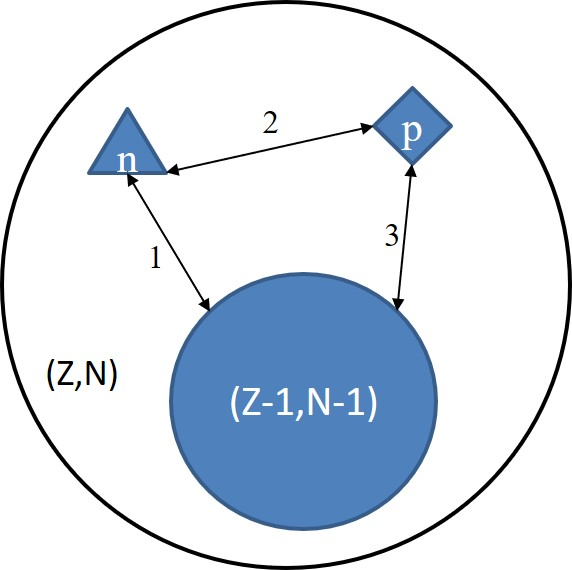
\includegraphics[width=0.5\textwidth]{figure/picV1p1n.jpg}
\caption{$V_{1p1n}(Z,N)$相互作用的基本图像.\label{picV1p1n}}
\end{figure}
这个公式是文献中提出的,为了理解这个公式,我们通过分离能$S_{p}(Z,N)$、$S_{n}(Z,N)$、$S_{1p-1n}(Z,N)$(其中分离能$S_{1p-1n}(Z,N)$在教科书中没有直接给出,只是我们对分离能的公式做了一个简单的推广(不知道这样的推广是否合理))所构成的3个一阶线性方程组:
\begin{displaymath}
\left\{ \begin{array}{l}
S_p(Z,N)=B(Z,N)-B(Z-1,N)\to1+2\\
S_n(Z,N)=B(Z,N)-B(Z-1,N)\to2+3\\
S_{1p1n}(Z,N)=B(Z,N)-B(Z-1,N-1)\to1+2+3
\end{array} \right.
\end{displaymath}
求解这个线性方程组就可以得到公式\ref{eq_V1p1n}。
\begin{figure}[H]
\centering
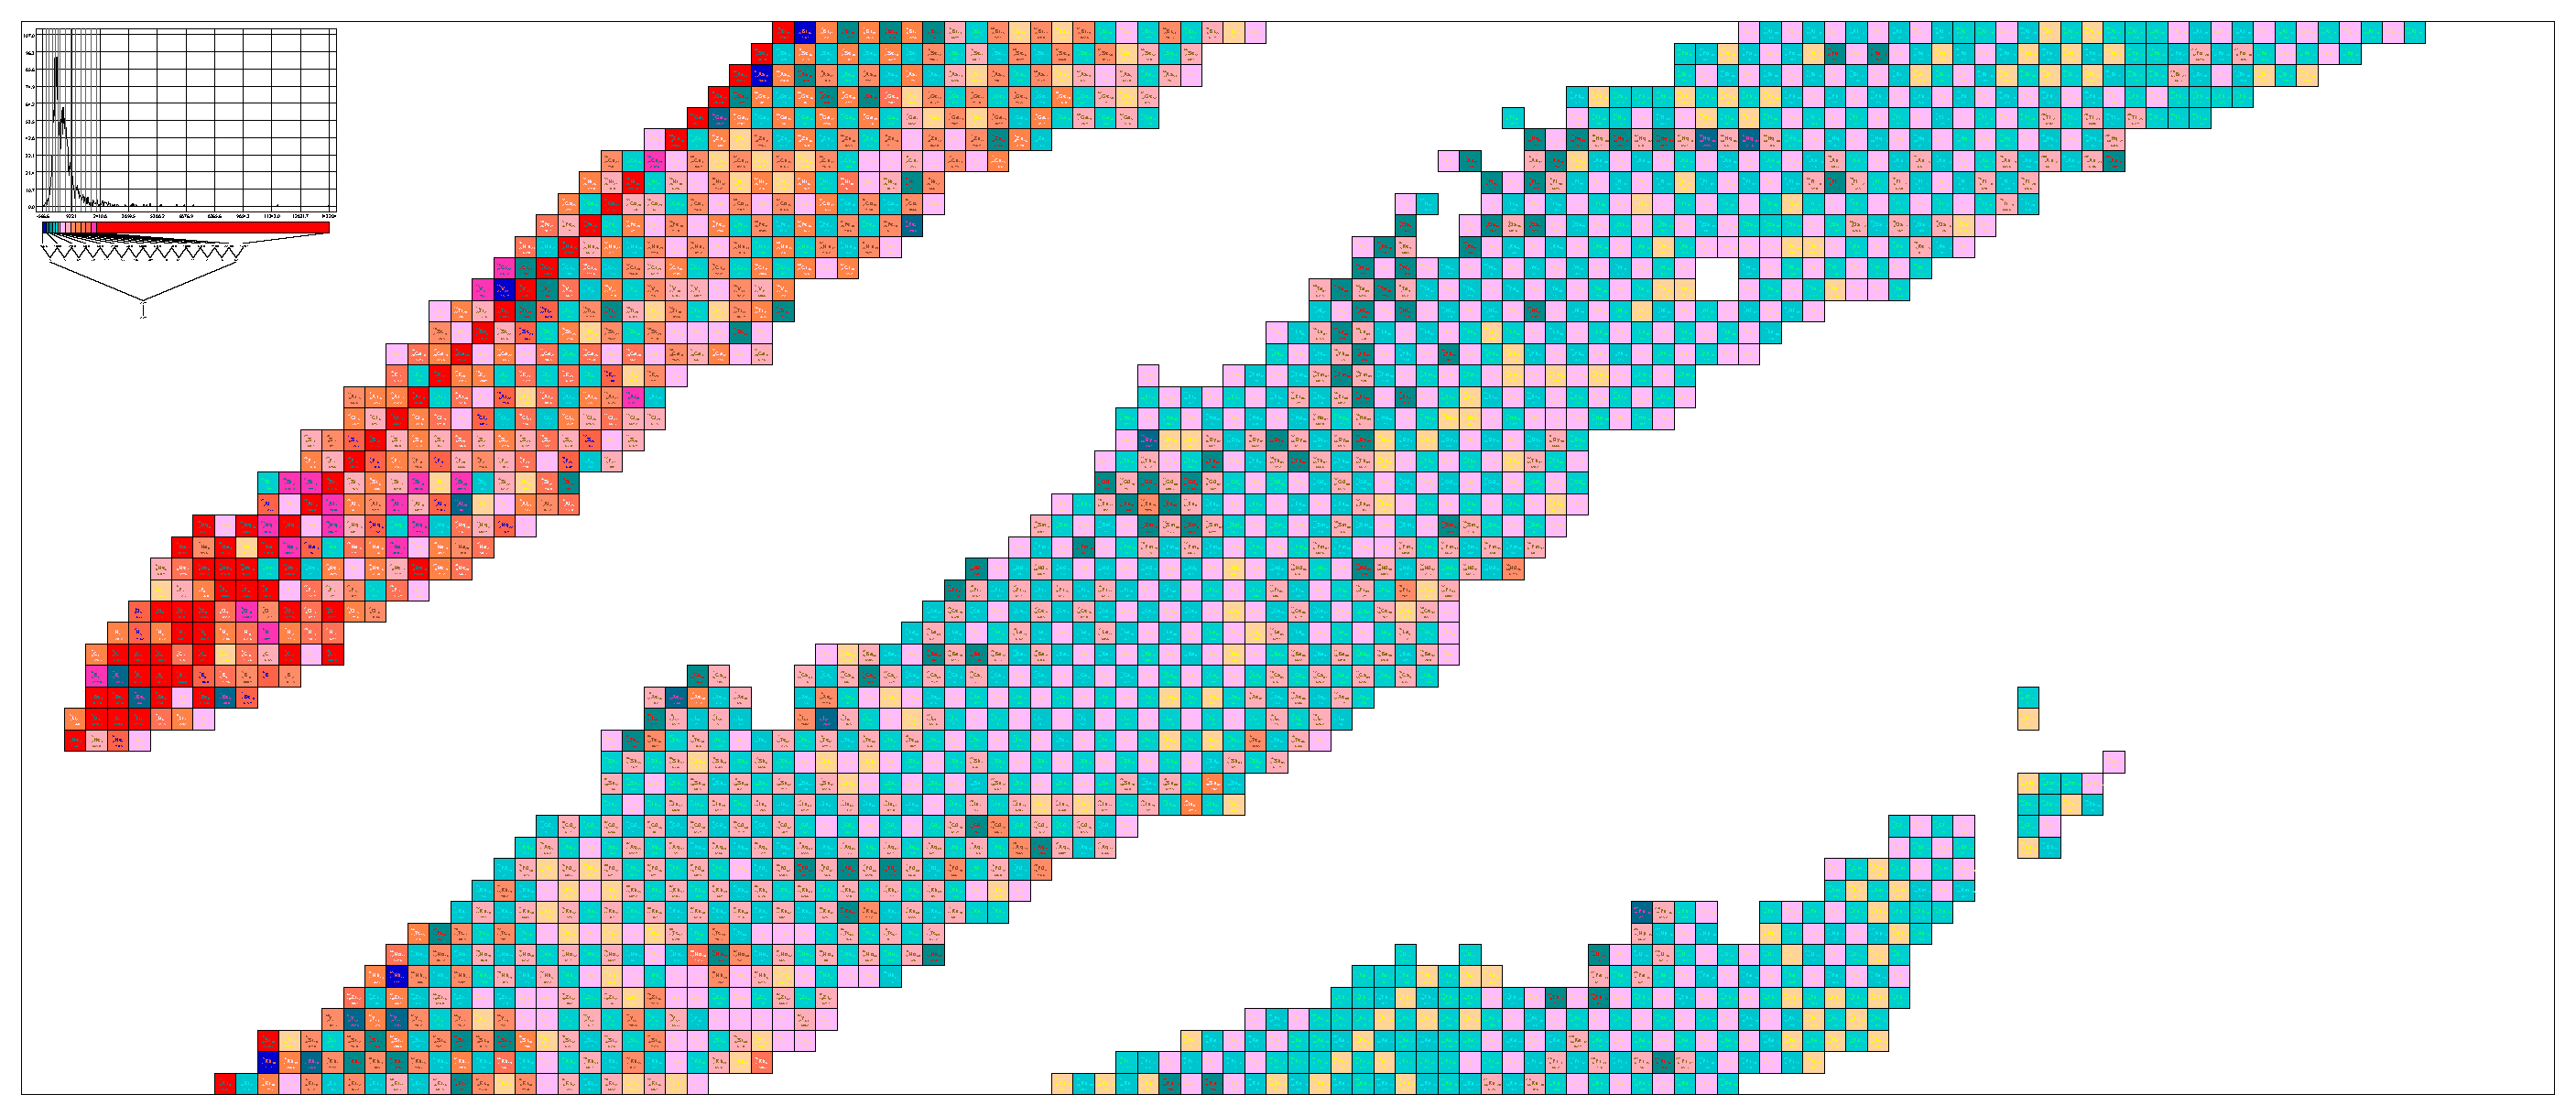
\includegraphics[width=0.9\textwidth]{figure/oV1p1n.pdf}
\caption{mass-date-based $V_{1p-1n}(Z,N)$相互作用在核素图中的分布.\label{fig_oV1p1n}}
\end{figure}
\noindent从图 \ref{fig_oV1p1n}中我们可以直接观察到的特征有:
\begin{enumerate}
  \item 偶A核的$V_{1p-1n}(Z,N)$相互作用几乎都大于奇A核;
  \item N=Z的核子的$V_{1p-1n}(Z,N)$相互作用都较大;
  \item N=Z附近的镜像核的$V_{1p-1n}(Z,N)$相互作用具有很好的对称性。
\end{enumerate}
\subsection{$V_{ip-jn}$相互作用}
在文献中我们也看到了描述原子核最外层的质子中子之间相互作用的更一般的公式:
\begin{eqnarray}
  V_{ip-jn}(Z,N)&=&B(Z,N)-B(Z-i,N)\nonumber\\
  &-&B(Z,N-j)+B(Z-i,N-j) \label{eq.Vipjn}
\end{eqnarray}
我们可以证明$V_{1p-1n}(Z,N)$与$V_{ip-jn}$存在着如下的关系:
\begin{eqnarray}
  &\ &V_{ip-jn}(Z,N)\nonumber\\
  &=&V_{1p-jn}(Z,N)+V_{1p-jn}(Z-1,N)+\cdots+V_{1p-jn}(Z-i+1,N)\nonumber\\
  &=&V_{1p-1n}(Z,N)+V_{1p-1n}(Z,N-1)+\cdots+V_{1p-1n}(Z,N-j+1)\nonumber\\
  &\ &+V_{1p-1n}(Z-1,N)+V_{1p-1n}(Z-1,N-1)+\cdots+V_{1p-1n}(Z-1,N-j+1)\nonumber\\
  &\ &\qquad\qquad\qquad\qquad\qquad\qquad\vdots\nonumber\\
  &\ &+V_{1p-1n}(Z-i+1,N)+V_{1p-1n}(Z-i+1,N-1)\nonumber\\
  &\ &\quad+\cdots+V_{1p-1n}(Z-i+1,N-j+1)\label{eq.Vpn}
\end{eqnarray}
由此可以直接得到两个结论:
\begin{enumerate}
\item 所有由$V_{ip-jn}(Z,N)(i\ or\ j>1)$所得到的规律都可以归结为$V_{1p-1n}(Z,N)$的规律.\ (可以将其他人所提出的 $V_{ip-jn}(Z,N)(i\ or\ j>1)$规律都总结为  $V_{1p-1n}(Z,N)$ 的规律)
\item 由于这样提取的$n-p$相互作用完全无法考虑外层核子对内层核子的影响,所有这只是对真实$n-p$ 相互作用的一个极大的近似.\
\end{enumerate}

\subsection{同类核子间的相互作用}
同类核子间的相互作用包括配对核子间的对关联效应,以及未配对核子间的相互作用,其中同类核子间的对关联效应已经得到了广泛的研究,其mass-date-based $P_p(Z,N)$、$P_n(Z,N)$相互作用的公式\cite{RN560}:
\begin{eqnarray}
  V_p(Z,N)&=&S_p(Z,N)-S_p(Z-1,N)\\
  &=&[B(Z,N)-B(Z-1,N)]-[B(Z-1,N)-B(Z-2,N)]\quad \textrm{for even Z}\nonumber
\end{eqnarray}
以及
\begin{eqnarray}\label{eq_Pn}
  V_n(Z,N)&=&S_n(Z,N)-S_n(Z,N-1)\\
  &=&[B(Z,N)-B(Z,N-1)]-[B(Z,N-1)-B(Z,N-2)]\quad \textrm{for even N}\nonumber
\end{eqnarray}
以$P_n(Z,N)$相互作用为例,其基本物理图像可以看作:
\begin{figure}[H]
\centering
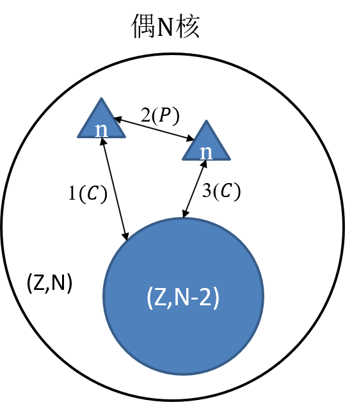
\includegraphics[width=0.5\textwidth]{figure/zV1n1ne.png}
\caption{偶N核的mass-date-based $P_n(Z,N)$相互作用的基本图像.\label{fig_zV1n1ne}}
\end{figure}
\noindent其中$P$表示偶N核最外层配对的中子之间的对关联作用,$C$表示外层的中子与内层的核心之间的相互作用,那么公式\ref{eq_Pn}就对应着:
\begin{eqnarray}
  V_n(Z,N)&=&S_n(Z,N)-S_n(Z,N-1)\\ \nonumber
  &\to&1(C)+2(P)-3(C)\\ \nonumber
  &\to&P\quad \textrm{for even N}\nonumber
\end{eqnarray}
这从基本的图像上说明了为什么这个公式可以计算得到对关联相互作用。图\ref{fig_oV1n1n}给出了其在核素图中的分布:
\begin{figure}[H]
\centering
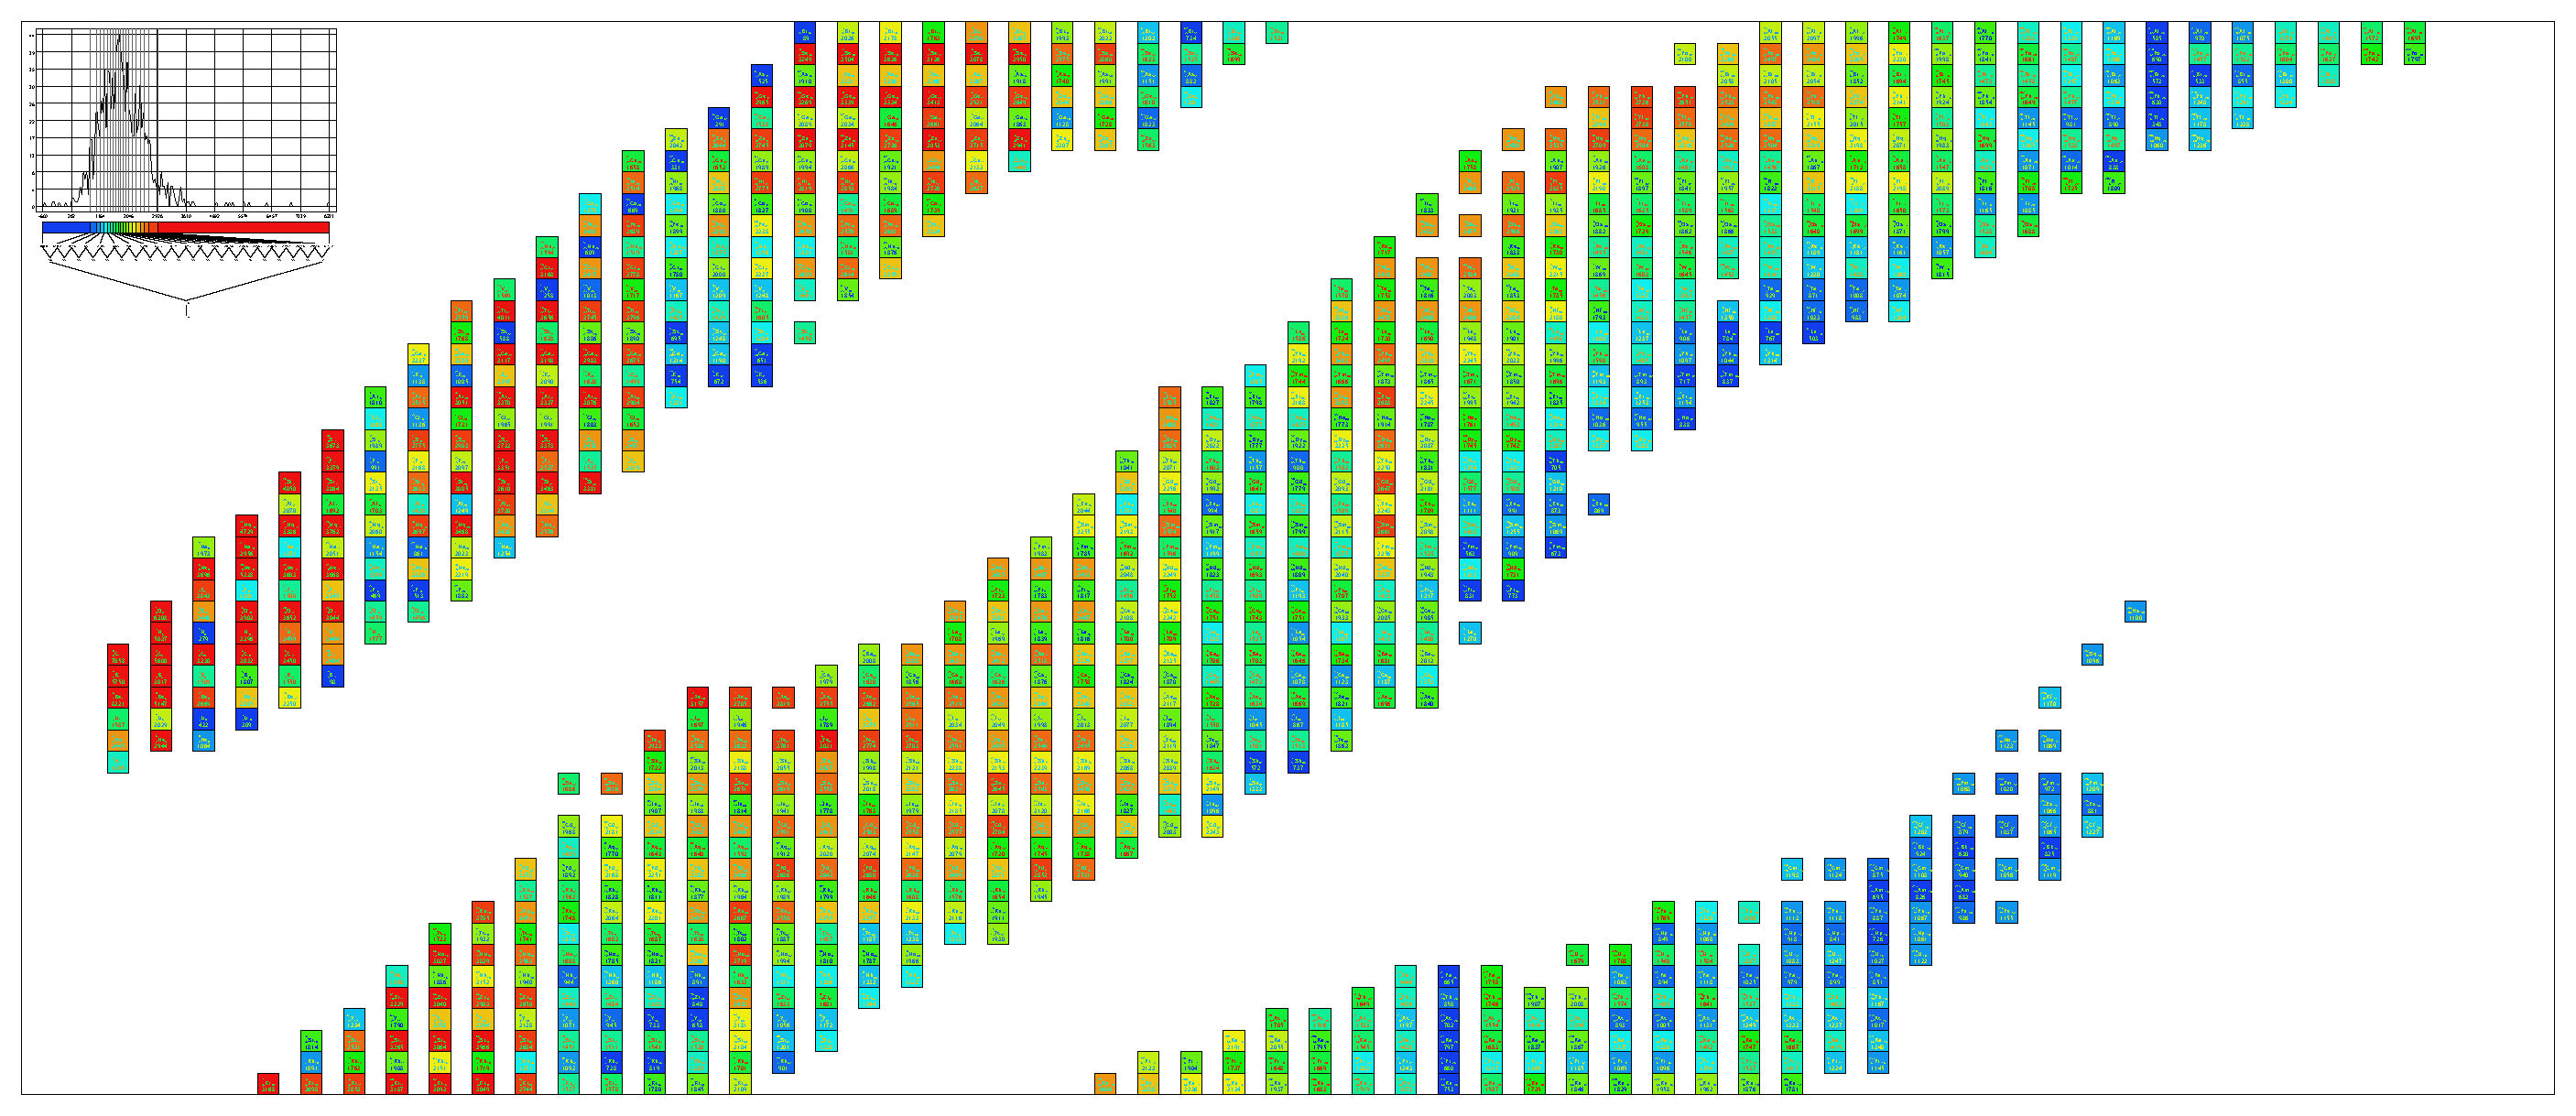
\includegraphics[width=0.9\textwidth]{figure/expVPn50eN.pdf}
\caption{偶N核的最外层配对核子之间的相互作用在核素图中的分布.\label{fig_expVPn50eN}}
\end{figure}
\begin{figure}[H]
\centering
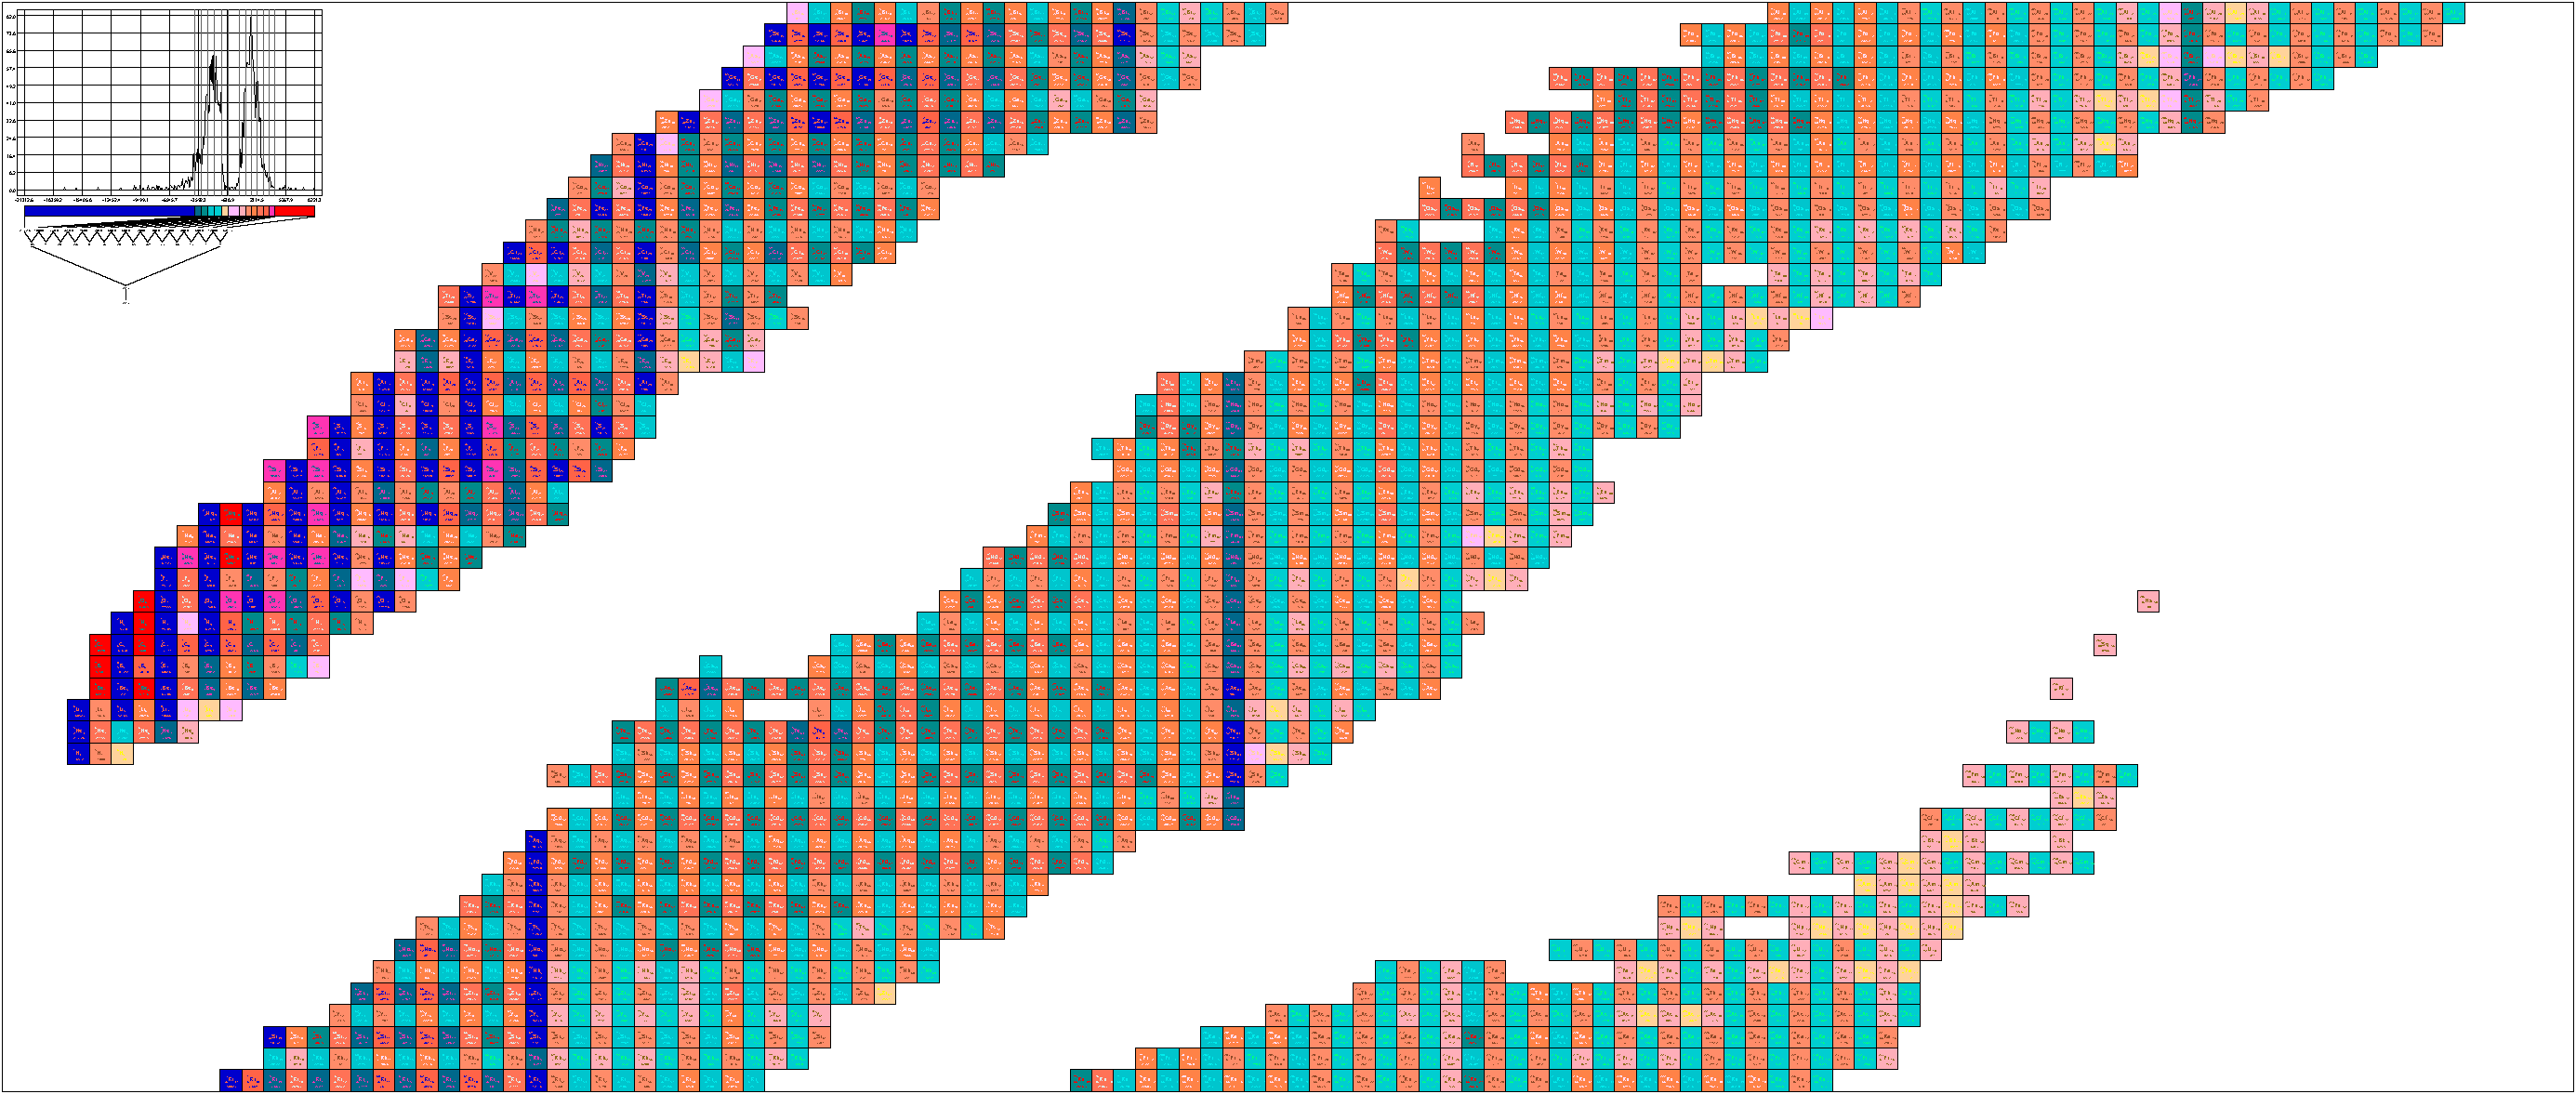
\includegraphics[width=0.9\textwidth]{figure/oV1n1n.pdf}
\caption{利用公式\ref{eq_Pn}对所有核子计算的结果在核素图中的分布.\label{fig_oV1n1n}}
\end{figure}
在这个图中我们不仅给出了偶N核通过公式\ref{eq_Pn}计算得到的中子配对相互作用的分布,我们还给出了奇N核通过同样的公式计算给出的结果,从图中我们可以观察到:
\begin{enumerate}
  \item 偶N核的统计分布呈现一个不对称的峰型分布;
  \item 奇N核与偶N核的计算结果的统计分布基本关于零对称,但是奇N核略微向左偏离。
  \item 在$N>20$的质量区奇N核的计算结果在壳层附近(一般比幻数大1的地方)的数值明显比其他地方大,而偶N核却没有观察到这样的现象。
  \item 在$N>20$的质量区奇N核的计算结果在数值上明显比偶N核的大,呈现明显的奇偶效应。
\end{enumerate}

为了解释奇N核的这样的性质,我们对奇N核进行了分析,其基本图像见图\ref{fig_zV1n1no}:
\begin{figure}[H]
\centering
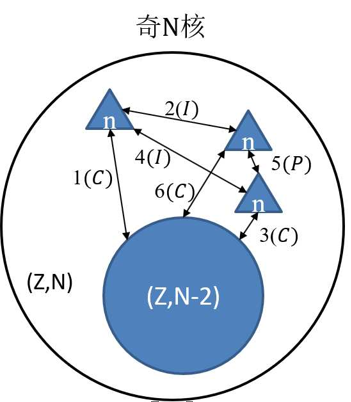
\includegraphics[width=0.5\textwidth]{zV1n1no.png}
\caption{奇N核的的基本图像.\label{fig_zV1n1no}}
\end{figure}
\noindent其中$I$表示奇N核的最外层的未配对核子与最外层的配对核子之间的相互作用,那么对比于前面的讨论,公式\ref{eq_Pn}在这里的含义是:
\begin{eqnarray}
V_n(Z,N)&=&S_n(Z,N)-S_n(Z,N-1)\quad \textrm{for odd N}\\ \nonumber
&\to&1(C)+2(I)+4(I)-[5(P)+6(C)]\\ \nonumber
&\to&2(I)+4(I)-5(P)\nonumber
\end{eqnarray}
如果我们认为最外层配对的中子之间的对关联作用$(P)$是要远大于奇N核的最外层的未配对核子与最外层的配对核子之间的相互作用$(I)$的,那么这就可以很好的解释奇N核与偶N核的计算结果的统计分布基本关于零对称,并且奇N核略微向左偏离的性质了。那么,我们也很容易通过这个这个公式得到最外层的未配对核子与最外层的配对核子之间的相互作用$I$的表达式:
\begin{eqnarray}\label{eq_In}
I_n(Z,N)&=&V_n(Z,N)+V_n(Z,N-1)\quad \textrm{for odd N}\\
&=&[S_n(Z,N)-S_n(Z,N-1)]+[S_n(Z,N-1)-S_n(Z,N-2)]\nonumber\\
&=&S_n(Z,N)-S_n(Z,N-2)\nonumber\\
&=&[B(Z,N)-B(Z,N-1)]-[B(Z,N-2)-B(Z,N-3)]\nonumber\\
&\to&2(I)+4(I)\nonumber
\end{eqnarray}
图\ref{fig_expVIn50oN}给出了奇N核最外层的未配对核子与最外层的配对核子之间的相互作用在核素图中的分布:
\begin{figure}[H]
\centering
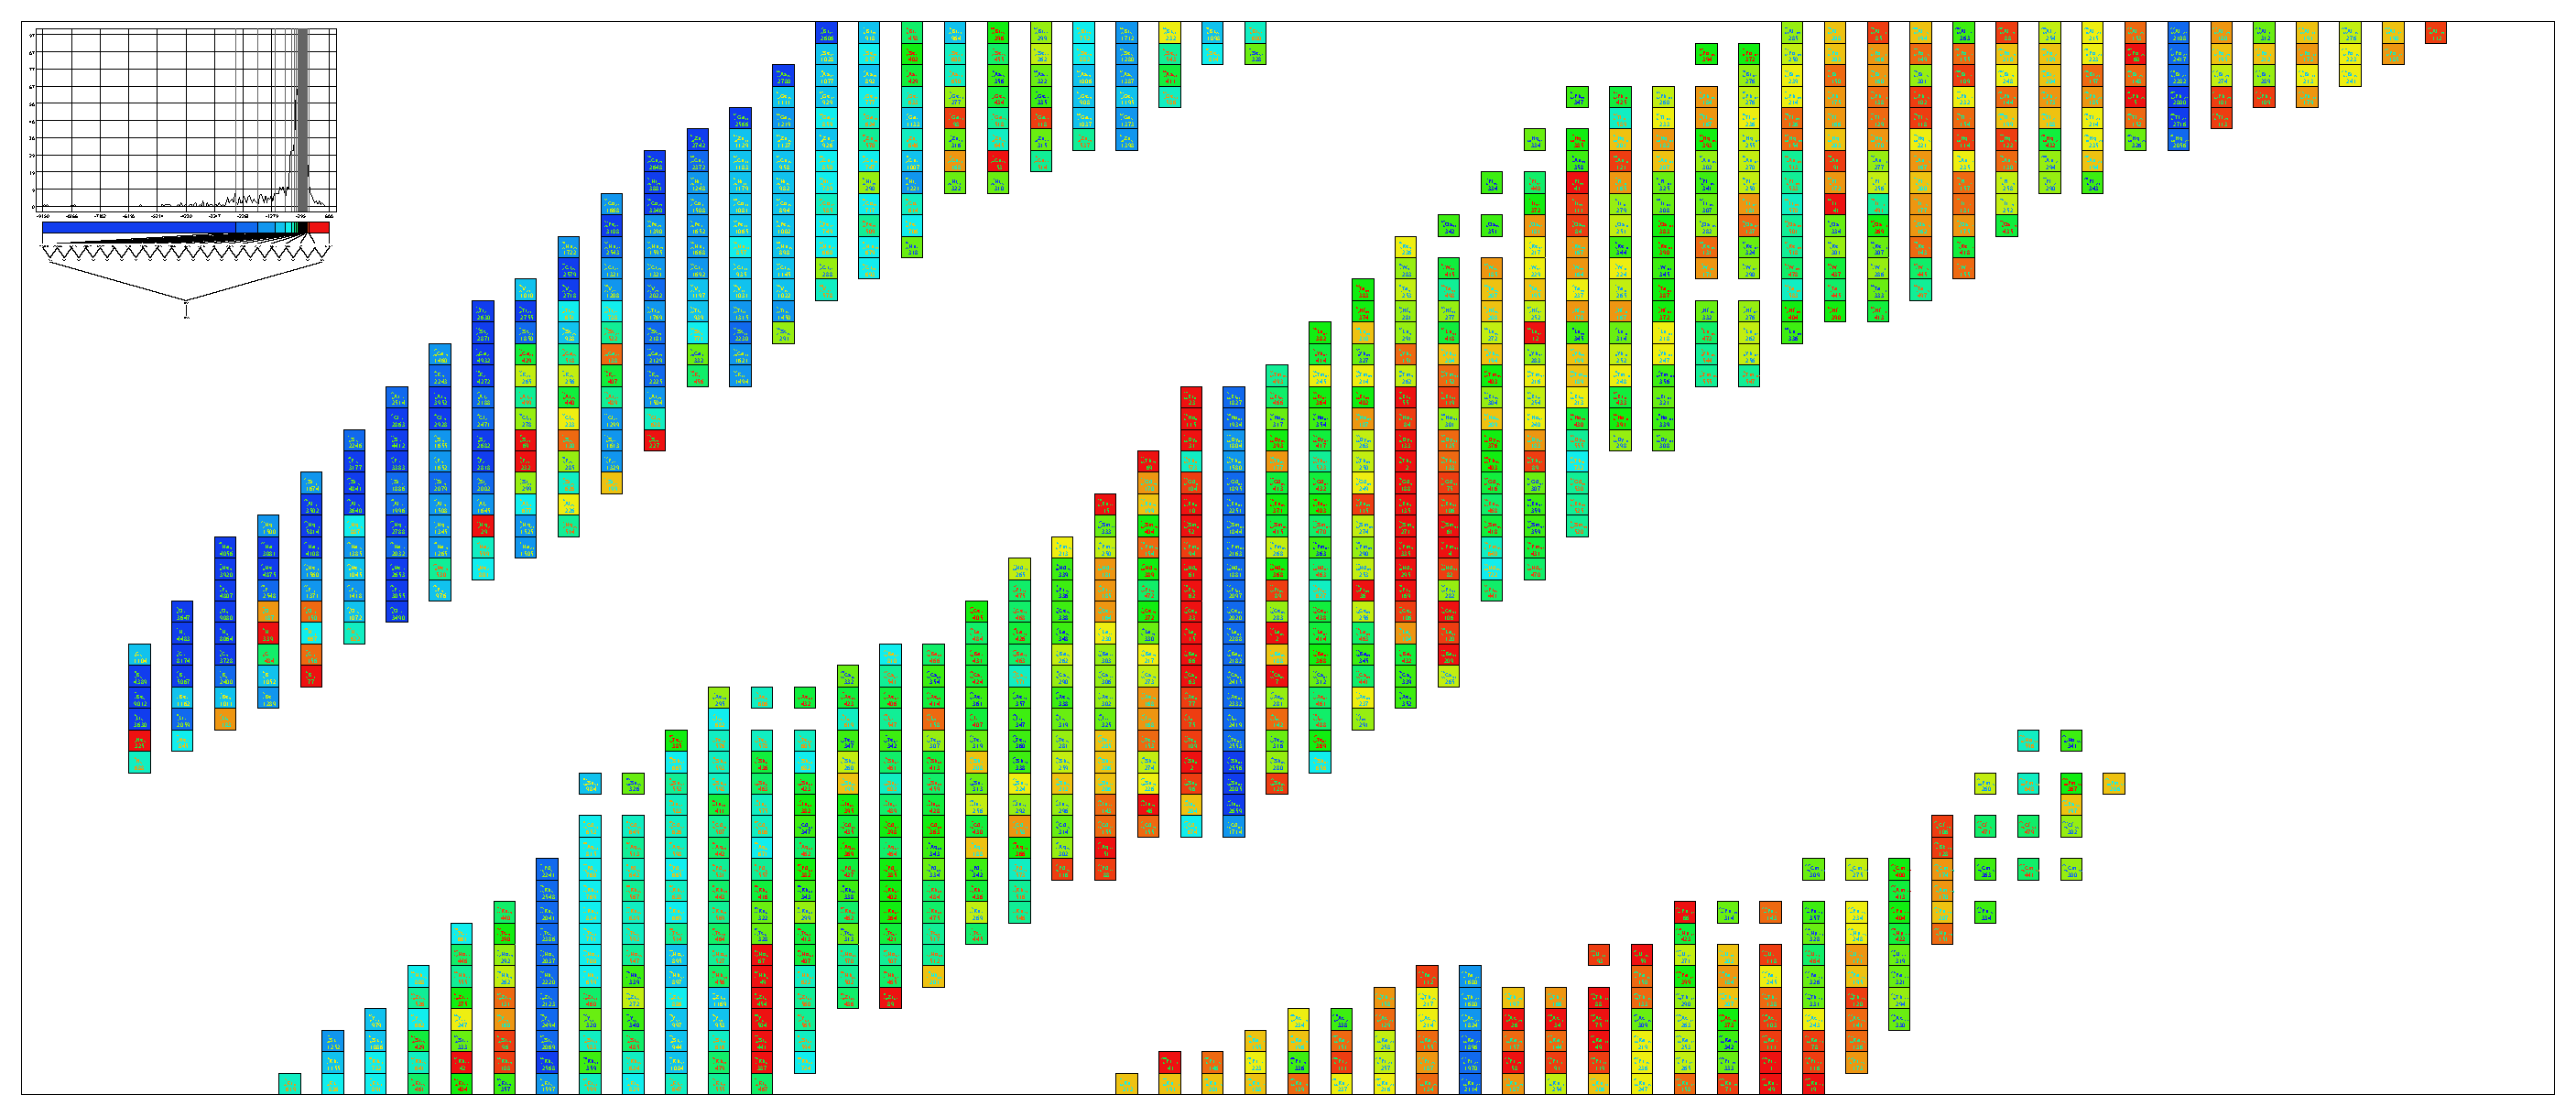
\includegraphics[width=0.9\textwidth]{expVIn50oN.pdf}
\caption{奇N核最外层的未配对核子与最外层的配对核子之间的相互作用在核素图中的分布.\label{fig_expVIn50oN}}
\end{figure}
\noindent 从这个图中我们可以明显的观察到中子数比幻数大1的奇N核的结果要比其它位置的相互作用要小得多,对比于图\ref{fig_expVPn50eN}我们似乎可以认为原子核的壳效应与核子的对关联之间没有直接的联系,壳效应是核子对之间的一种效应。
\section{mass-date-based相互作用的统计规律}
我们利用\href{http://amdc.impcas.ac.cn/web/masseval.html}{<The 2016 Atomic Mass Evaluation>}的数据计算mass-date-based interaction,并的到了他们随能量的统计分布,尝试了利用高斯分布以及类似于Yukawa势的表达式\ref{eq_fit}来拟合这样的统计分布。
\begin{equation}\label{eq_fit}
V=\left\{\begin{array}{ll}
10^{-a}(x-c)^d{\rm exp}\left[-\frac{d(x-c)^f}{f(b-c)^f}\right]&x>c\\
0&x\le c
\end{array}\right.
\end{equation}
其中$a,b,c,d,f$都是拟合参数。

首先得到的是$V_{1p-1n}(Z,N)$的统计分布,我们分析其可以很好的分解为奇A核和偶A核两种情况,并分别对其进行了拟合分析:
\begin{figure}[H]
\centering
\subfigure[利用公式\ref{eq_fit}对AME2016的偶A核的$V_{1p-1n}(Z,N)$相互作用进行的拟合.\label{fig_Y3FitV1p1neA50}]{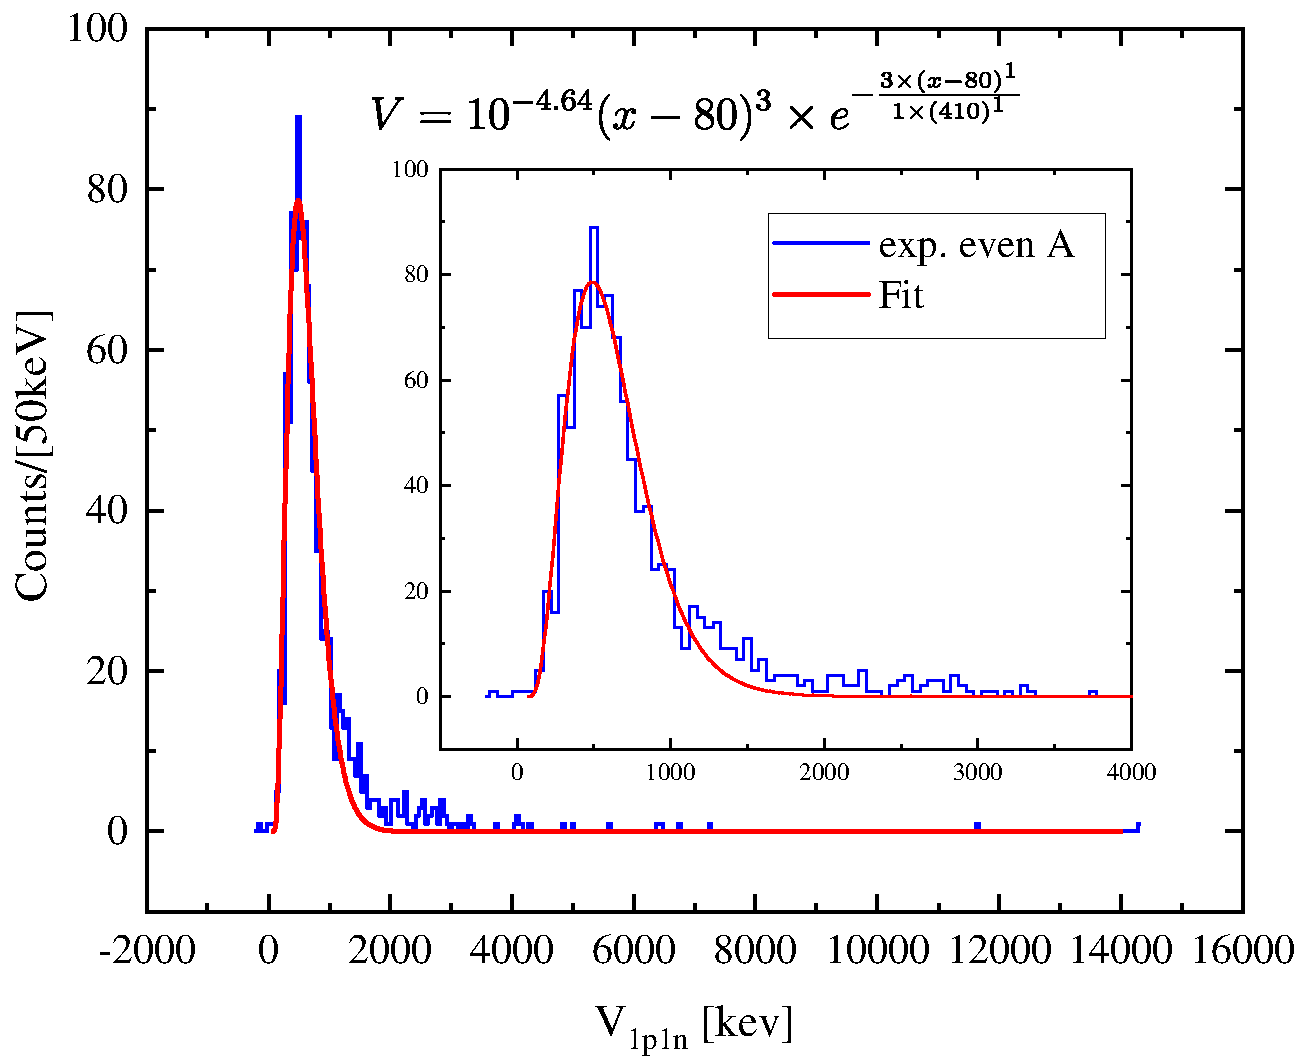
\includegraphics[width=0.4\textwidth]{figure/YE3fiteV1p1neA50.pdf}}
\qquad
\subfigure[利用公式\ref{eq_fit}对AME2016的奇A核的$V_{1p-1n}(Z,N)$相互作用进行的拟合.\label{fig_Y3FitV1p1noA50}]{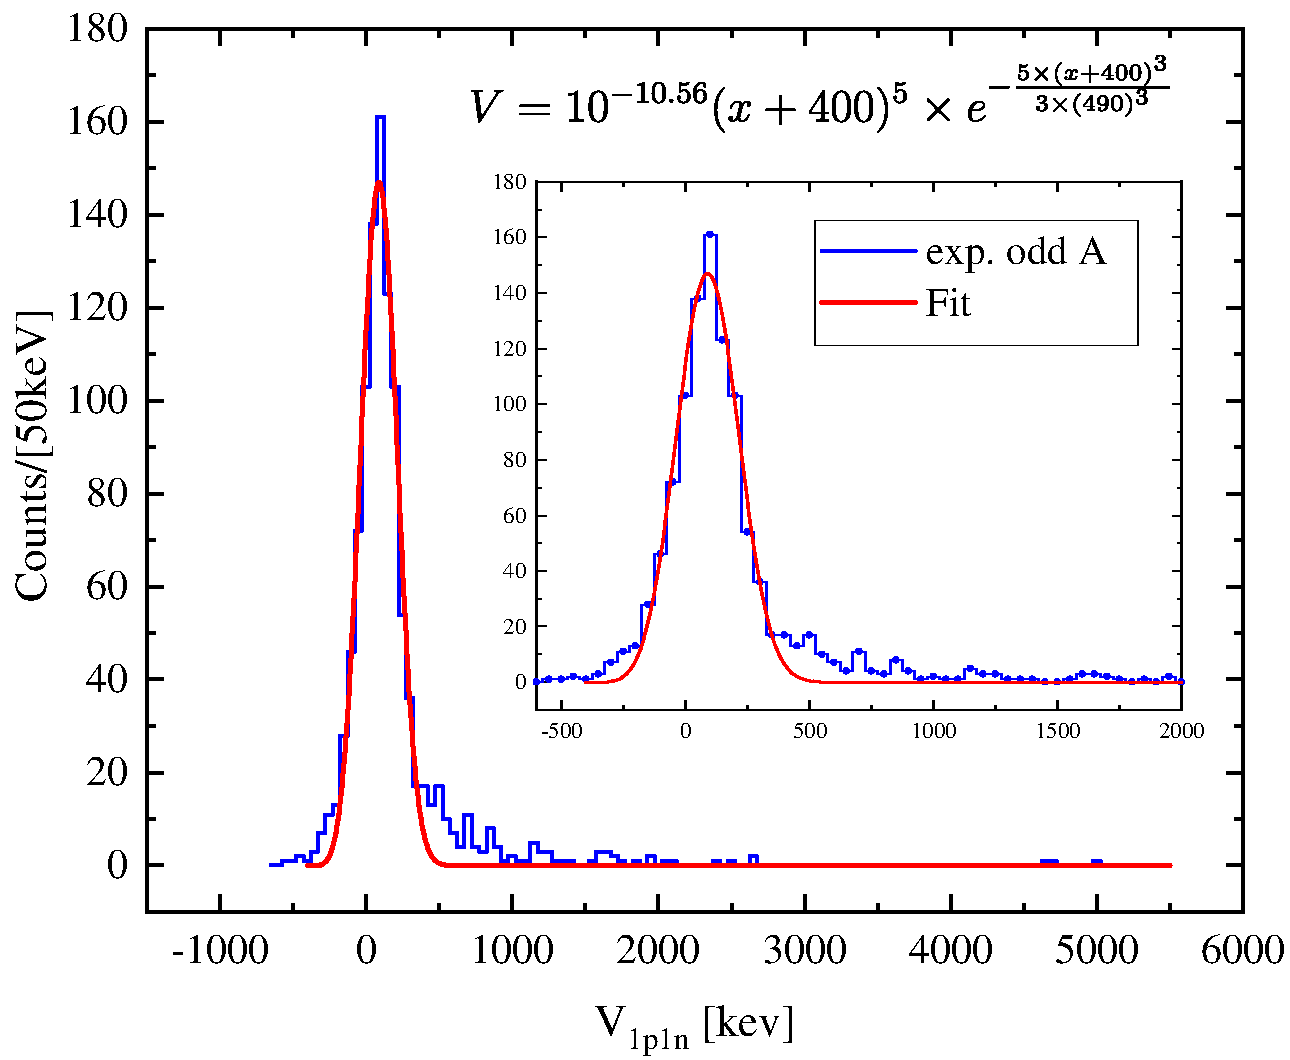
\includegraphics[width=0.4\textwidth]{figure/YE3fiteV1p1noA50.pdf}}
\caption{利用公式\ref{eq_fit}对AME2016的$V_{1p-1n}(Z,N)$相互作用的统计分布进行的拟合.\label{fig_YE3FitV1p2n_1}}
\end{figure}
\begin{figure}[H]
\centering
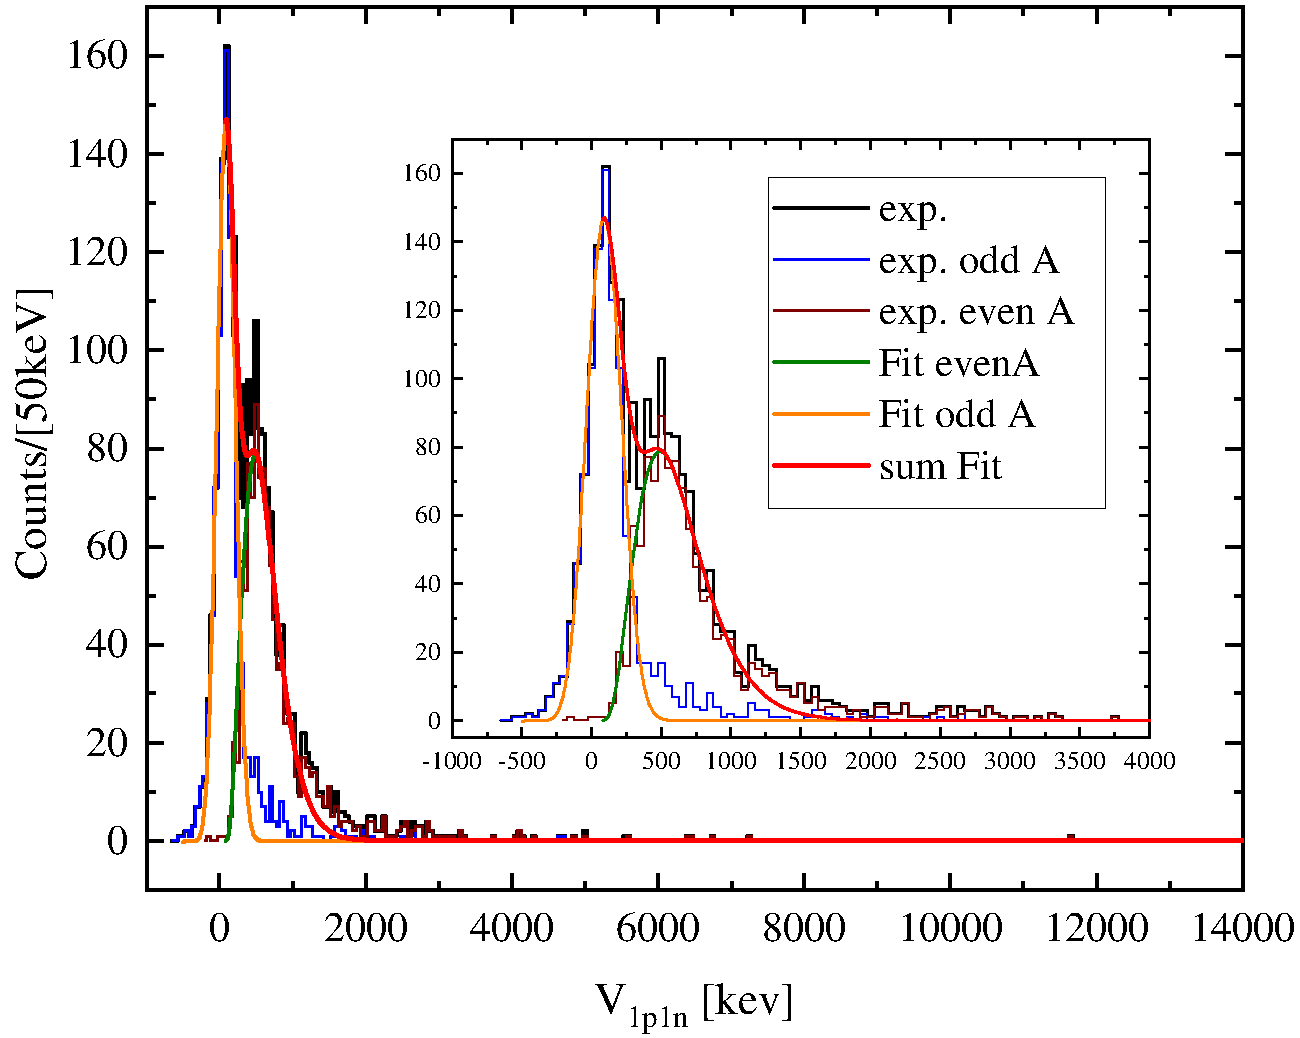
\includegraphics[width=0.6\textwidth]{figure/YE3fiteV1p1n50.pdf}
\caption{AME2016的奇A核的$V_{1p-1n}(Z,N)$相互作用的统计分布,以及拟合的结果.\label{fig_YE3fiteV1p1n50}}
\end{figure}

\begin{figure}[H]
\centering
\subfigure[利用公式\ref{eq_fit}对AME2016的偶A核的$V_{1p-2n}(Z,N)$相互作用进行的拟合.\label{fig_Y3FitV1p2neA50}]{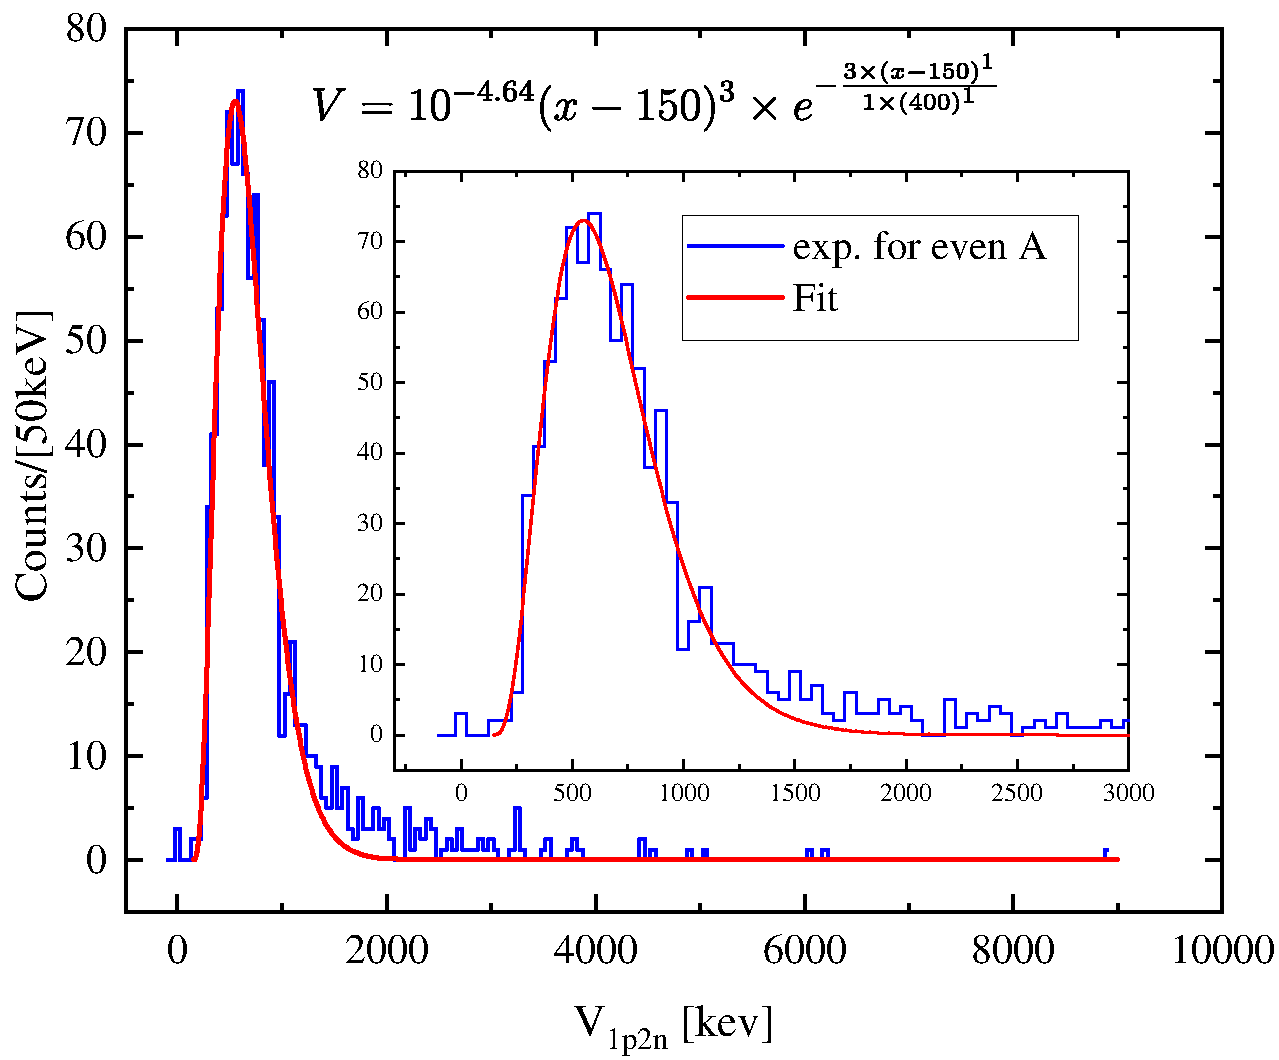
\includegraphics[width=0.4\textwidth]{figure/YE3fiteV1p2neA50.pdf}}
\qquad
\subfigure[利用公式\ref{eq_fit}对AME2016的奇A核的$V_{1p-2n}(Z,N)$相互作用进行的拟合.\label{fig_Y3FitV1p2noA50}]{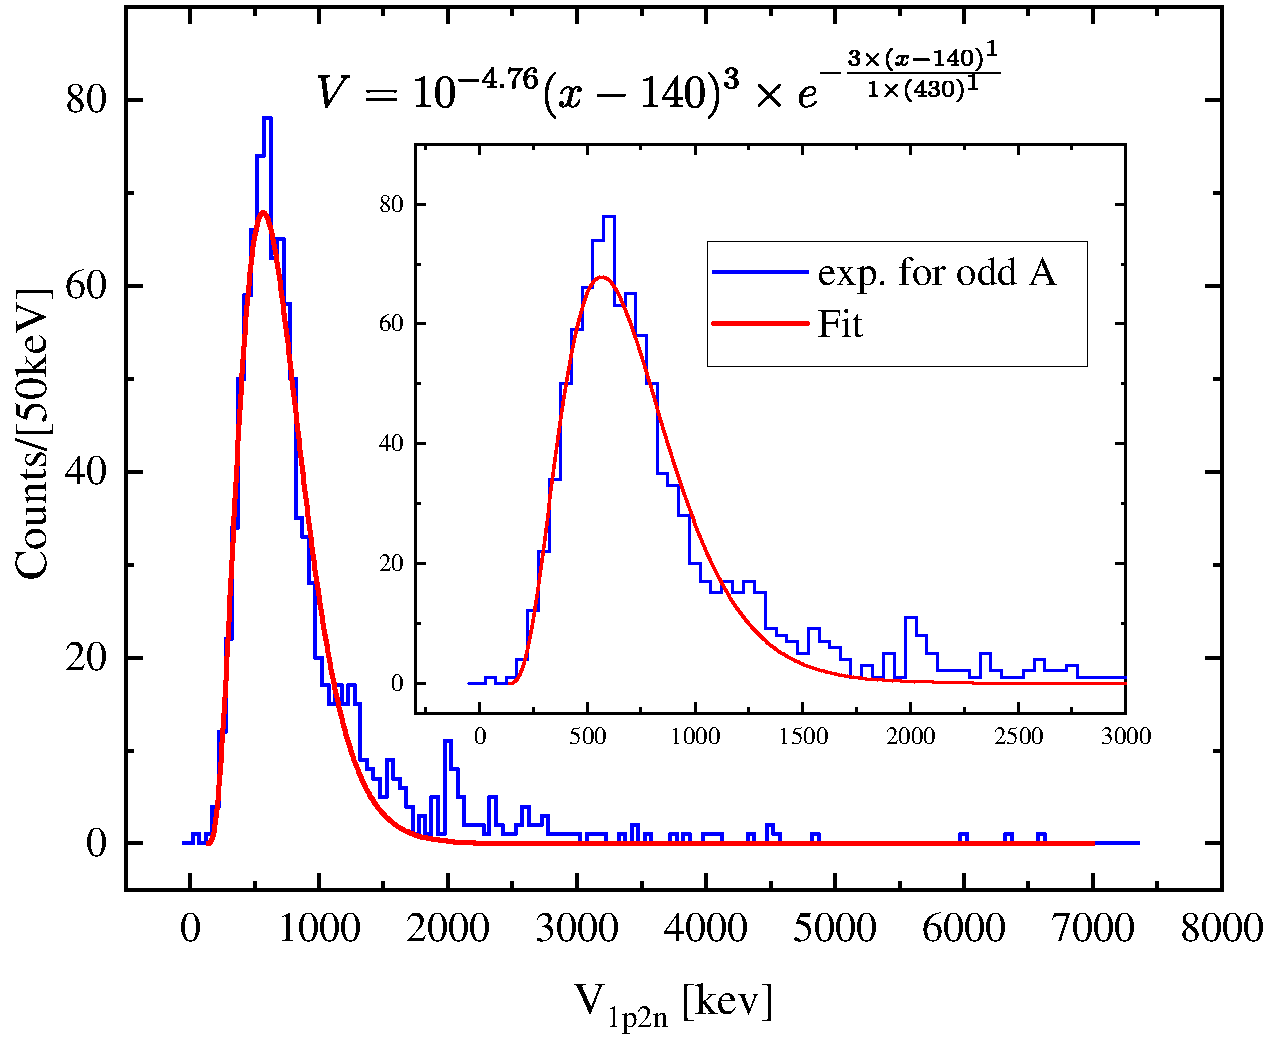
\includegraphics[width=0.4\textwidth]{figure/YE3fiteV1p2noA50.pdf}}
\caption{利用公式\ref{eq_fit}对AME2016的$V_{1p-2n}(Z,N)$相互作用的统计分布进行的拟合.\label{fig_YE3FitV1p2n_1}}
\end{figure}
\begin{figure}[H]
\centering
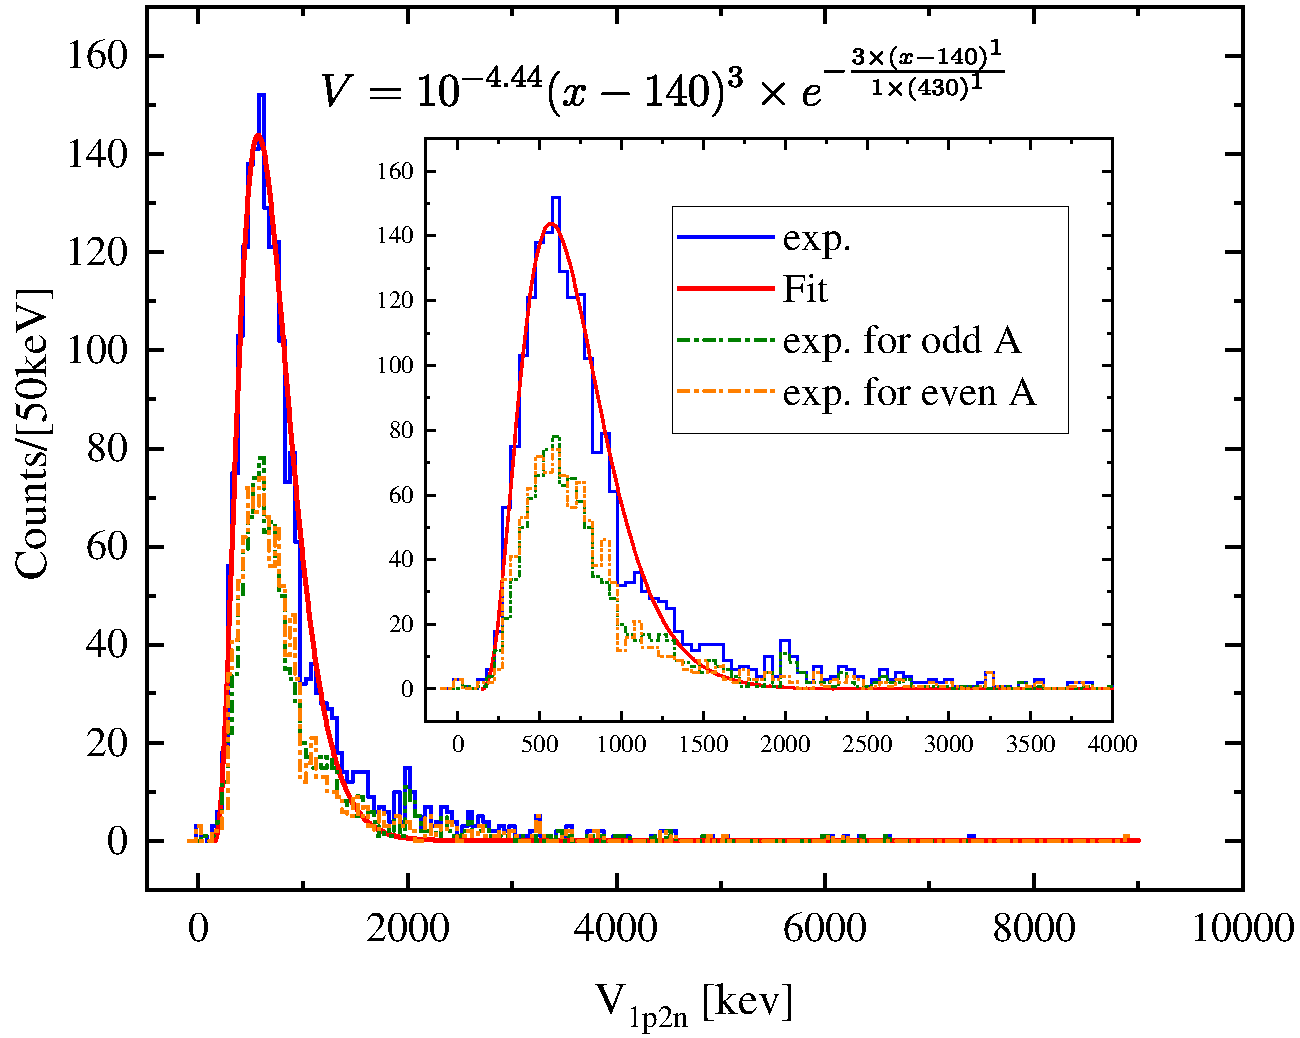
\includegraphics[width=0.6\textwidth]{figure/YE3fiteV1p2n50.pdf}
\caption{AME2016的奇A核的$V_{1p-2n}(Z,N)$相互作用的统计分布,以及拟合的结果.\label{fig_YE3fiteV1p2n50}}
\end{figure}

\begin{figure}[H]
\centering
\subfigure[利用公式\ref{eq_fit}对AME2016的偶A核的$V_{2p-1n}(Z,N)$相互作用进行的拟合.\label{fig_Y3FitV2p1neA50}]{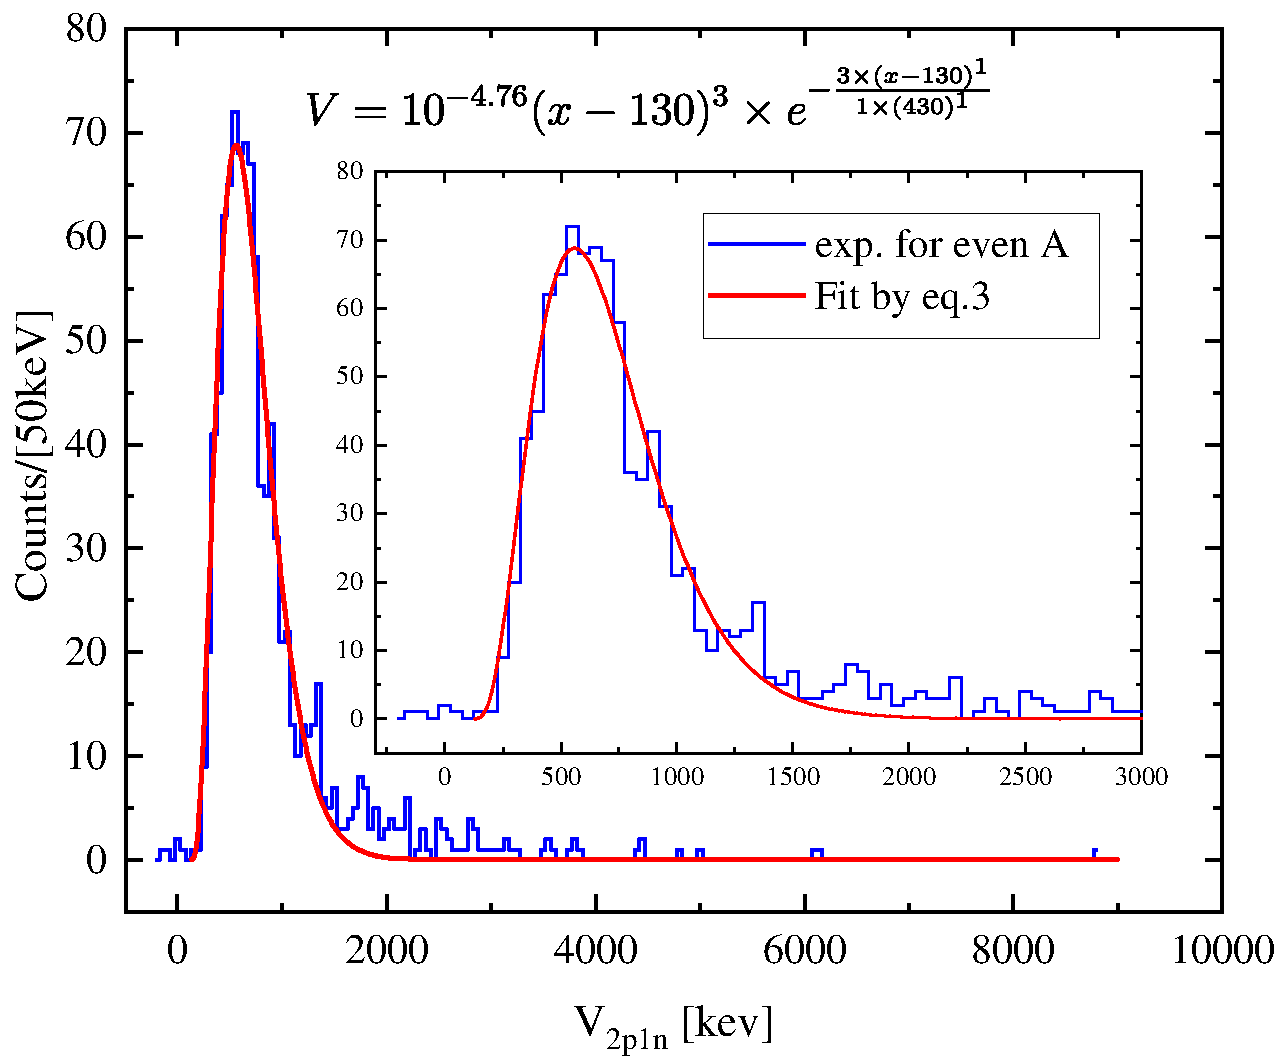
\includegraphics[width=0.4\textwidth]{figure/YE3fiteV2p1neA50.pdf}}
\qquad
\subfigure[利用公式\ref{eq_fit}对AME2016的奇A核的$V_{2p-1n}(Z,N)$相互作用进行的拟合.\label{fig_Y3FitV2p1noA50}]{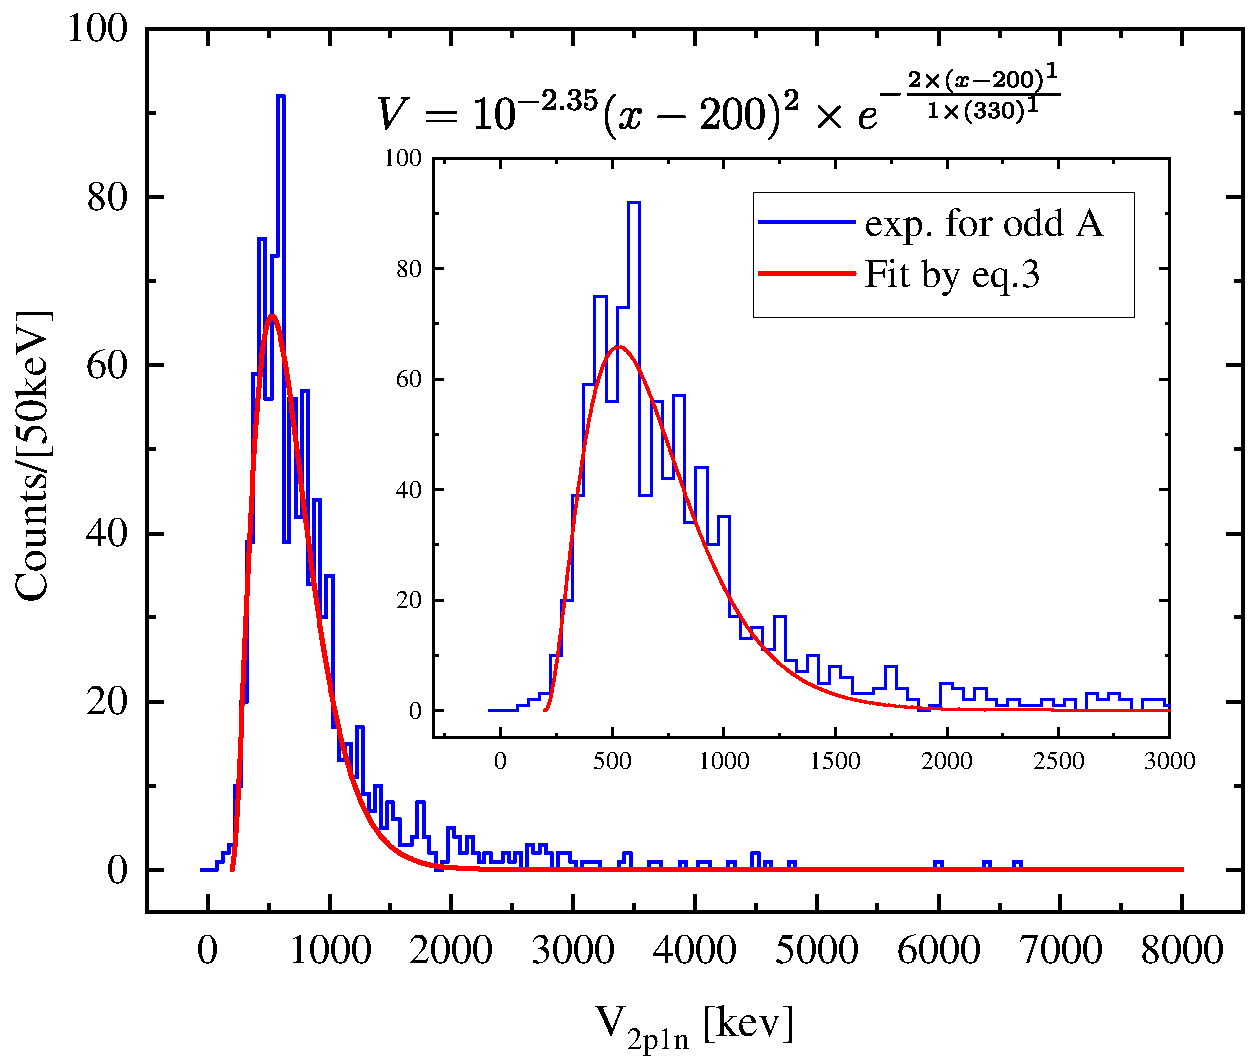
\includegraphics[width=0.4\textwidth]{figure/YE3fiteV2p1noA50.pdf}}
\caption{利用公式\ref{eq_fit}对AME2016的$V_{2p-1n}(Z,N)$相互作用的统计分布进行的拟合.\label{fig_YE3FitV2p1n_1}}
\end{figure}
\begin{figure}[H]
\centering
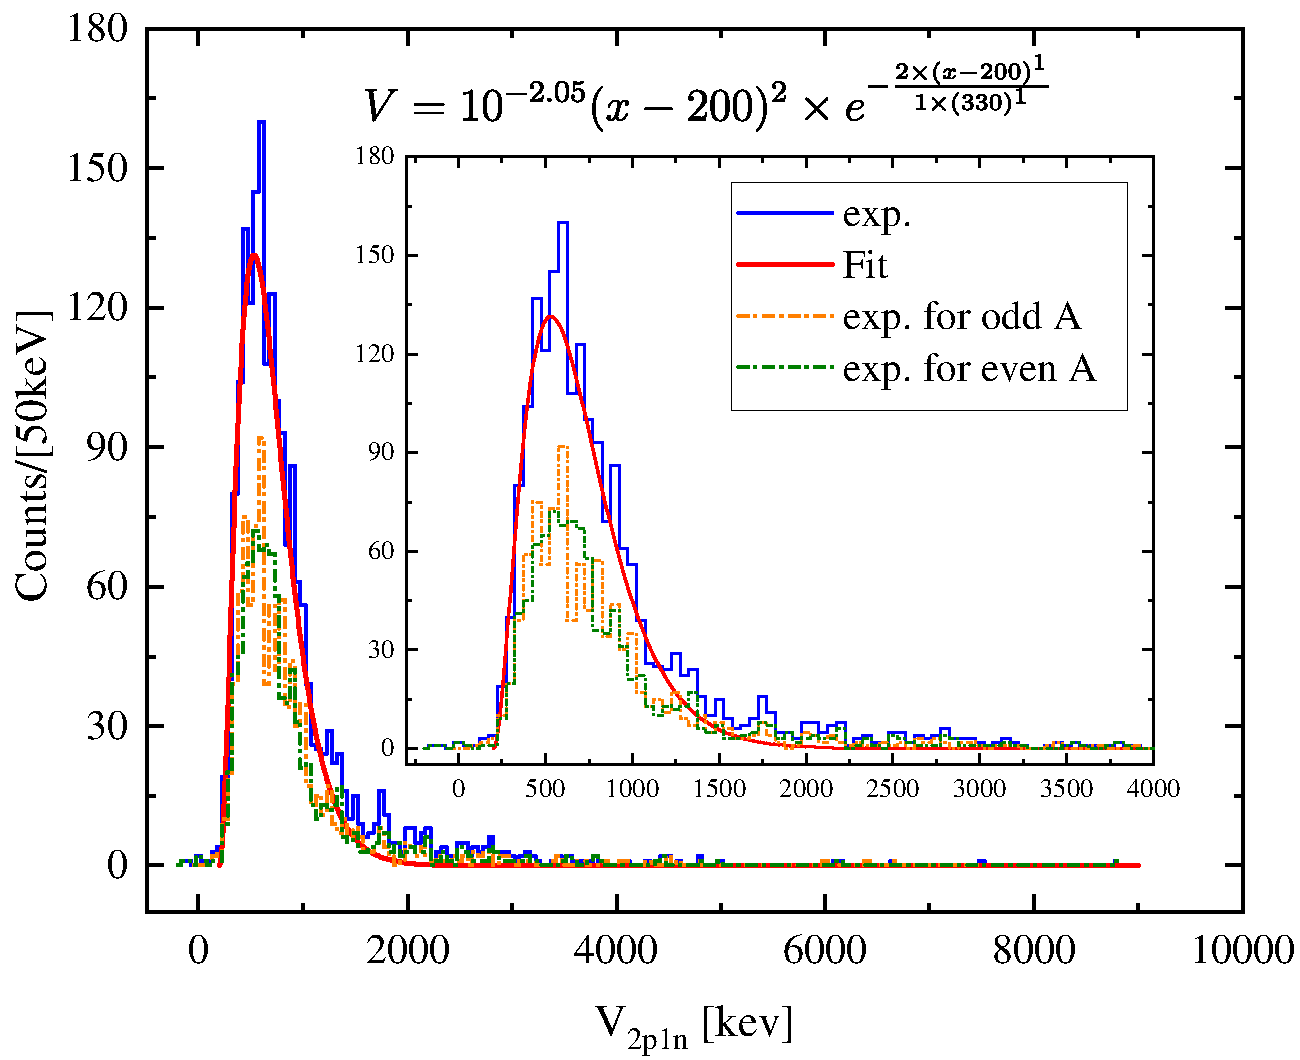
\includegraphics[width=0.6\textwidth]{figure/YE3fiteV2p1n50.pdf}
\caption{AME2016的奇A核的$V_{2p-1n}(Z,N)$相互作用的统计分布,以及拟合的结果.\label{fig_YE3fiteV2p1n50}}
\end{figure}

\begin{figure}[H]
\centering
\subfigure[利用公式\ref{eq_fit}对AME2016的偶A核的$V_{1p-3n}(Z,N)$相互作用进行的拟合.\label{fig_Y3FitV1p3neA100}]{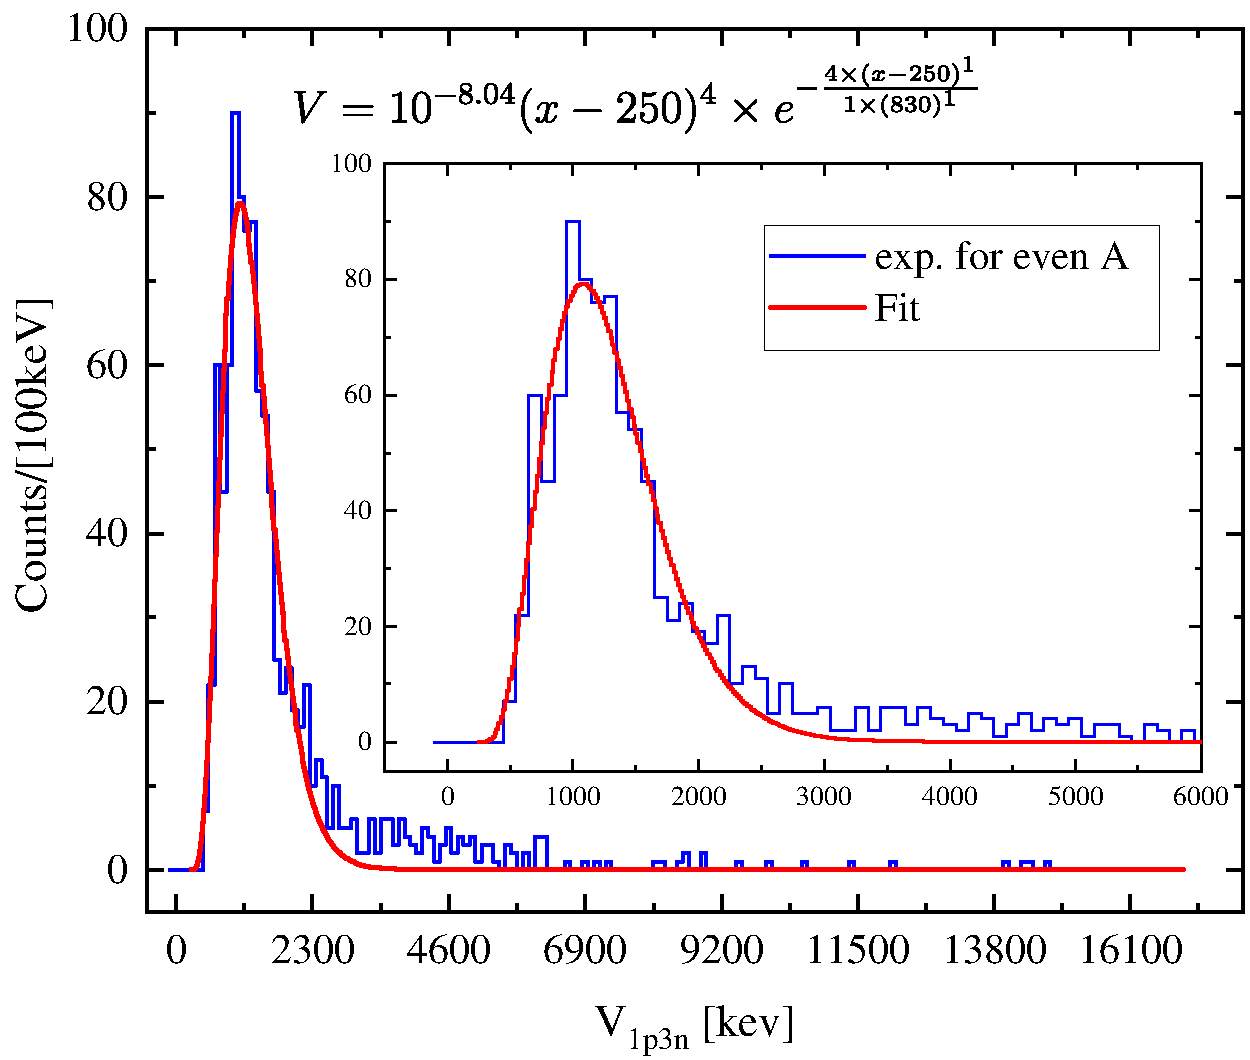
\includegraphics[width=0.4\textwidth]{figure/YE3fiteV1p3neA100.pdf}}
\qquad
\subfigure[利用公式\ref{eq_fit}对AME2016的奇A核的$V_{1p-3n}(Z,N)$相互作用进行的拟合.\label{fig_Y3FitV1p3noA100}]{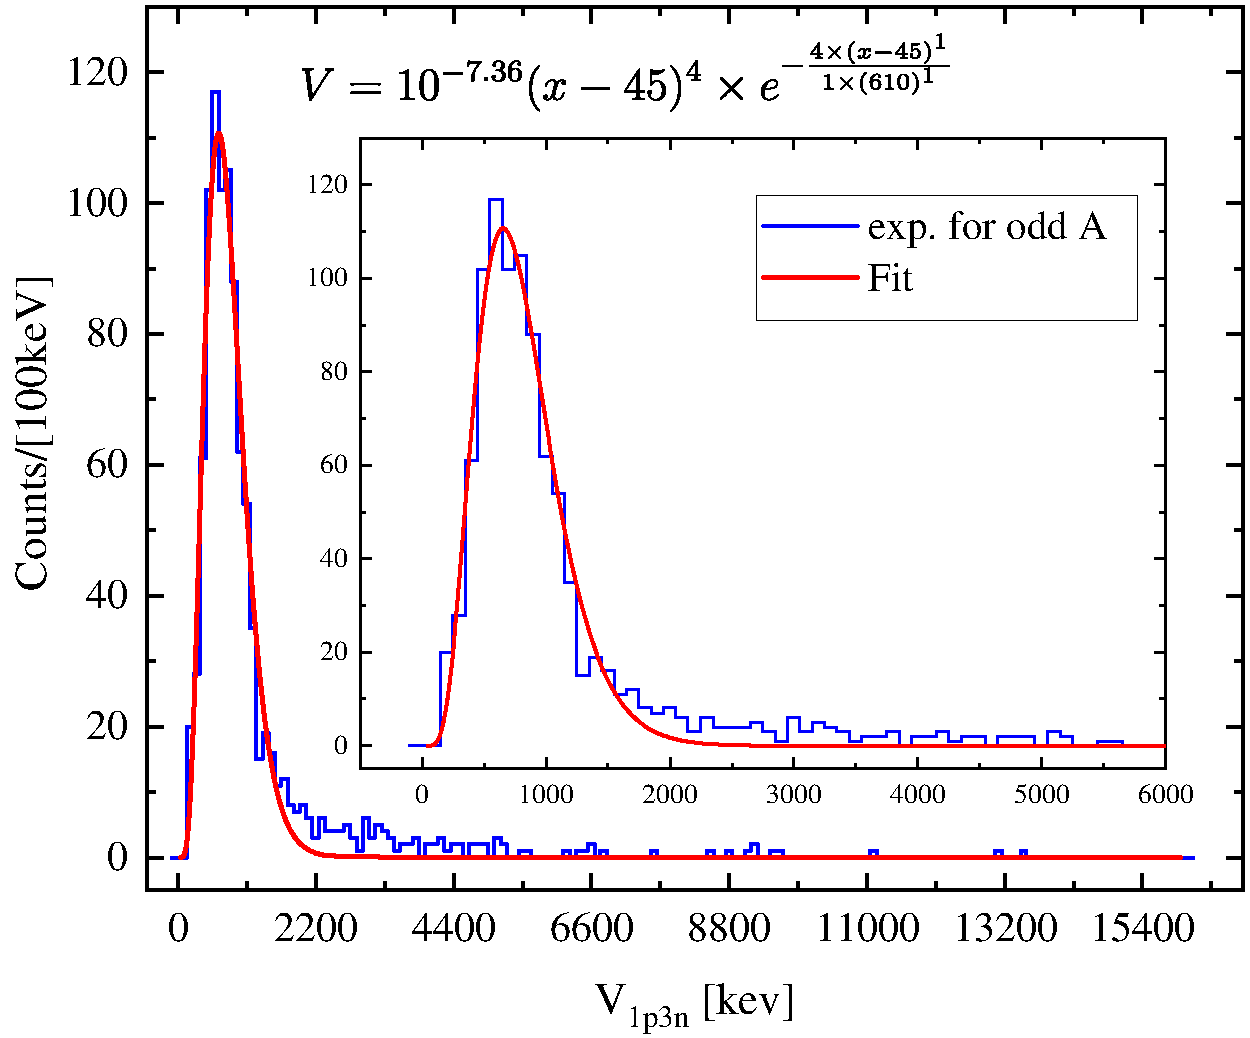
\includegraphics[width=0.4\textwidth]{figure/YE3fiteV1p3noA100.pdf}}
\caption{利用公式\ref{eq_fit}对AME2016的$V_{1p-3n}(Z,N)$相互作用的统计分布进行的拟合.\label{fig_YE3FitV1p3n_1}}
\end{figure}
\begin{figure}[H]
\centering
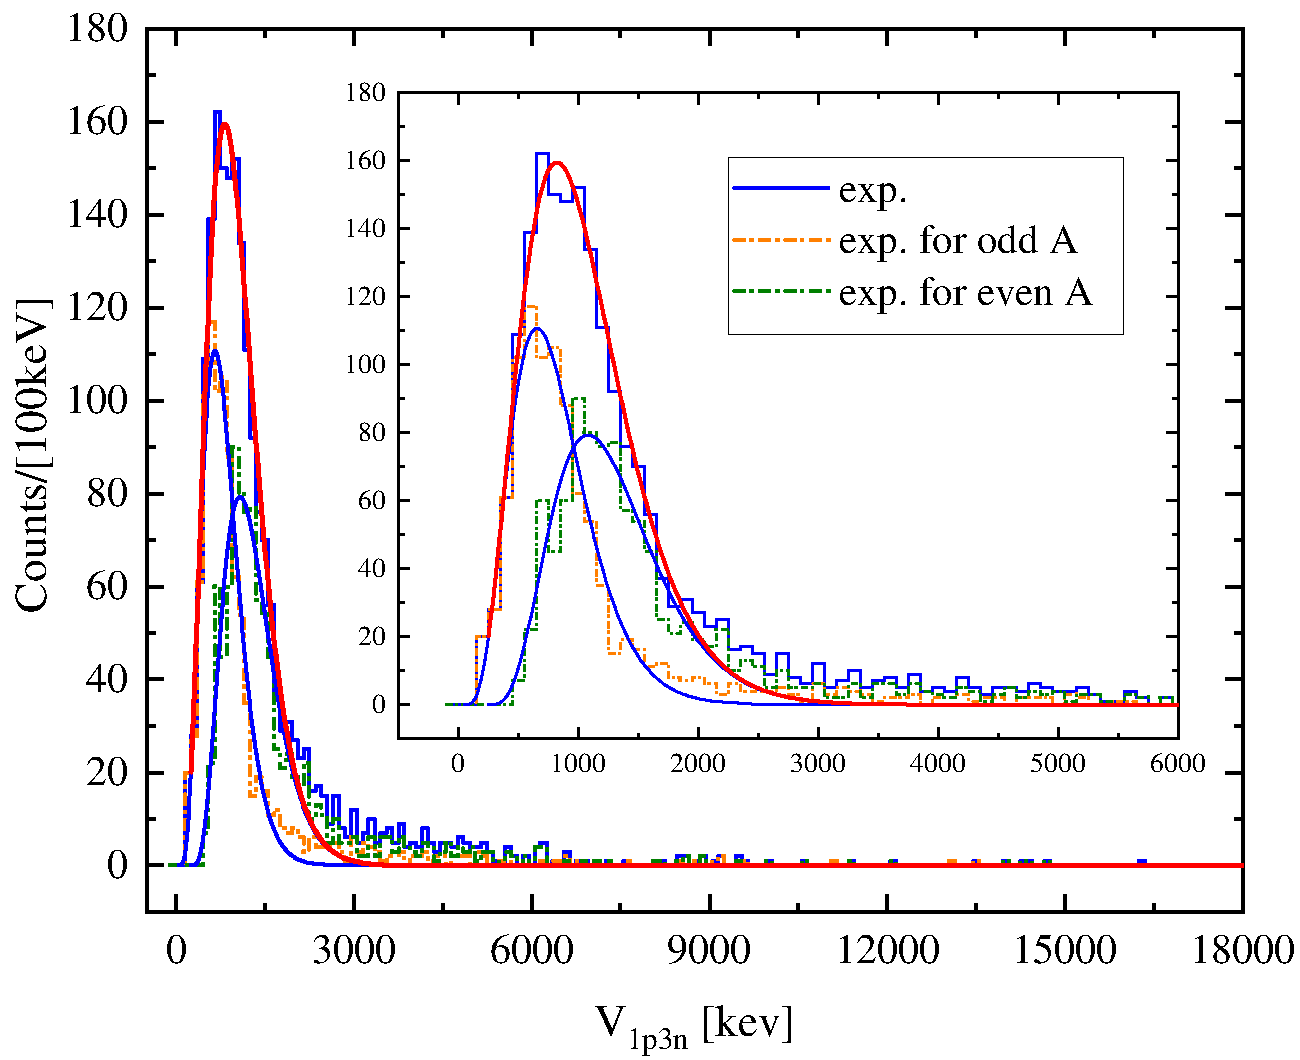
\includegraphics[width=0.6\textwidth]{figure/YE3fiteV1p3n100.pdf}
\caption{AME2016的奇A核的$V_{1p-3n}(Z,N)$相互作用的统计分布,以及拟合的结果.\label{fig_YE3fiteV1p3n100}}
\end{figure}

\begin{figure}[H]
\centering
\subfigure[利用公式\ref{eq_fit}对AME2016的偶A核的$V_{3p-1n}(Z,N)$相互作用进行的拟合.\label{fig_Y3FitV3p1neA100}]{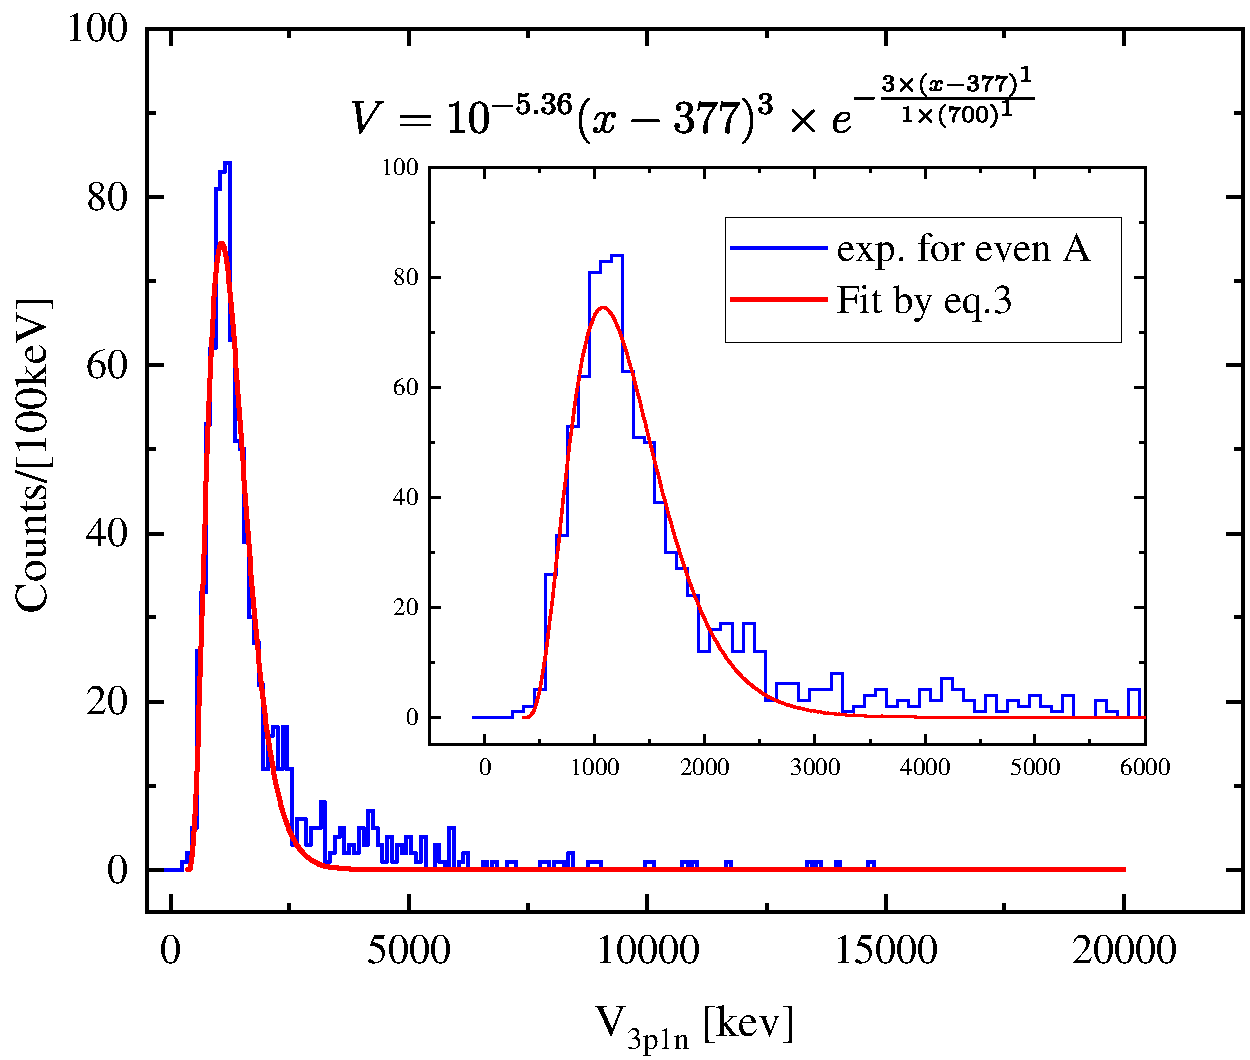
\includegraphics[width=0.4\textwidth]{figure/YE3fiteV3p1neA100.pdf}}
\qquad
\subfigure[利用公式\ref{eq_fit}对AME2016的奇A核的$V_{3p-1n}(Z,N)$相互作用进行的拟合.\label{fig_Y3FitV3p1noA100}]{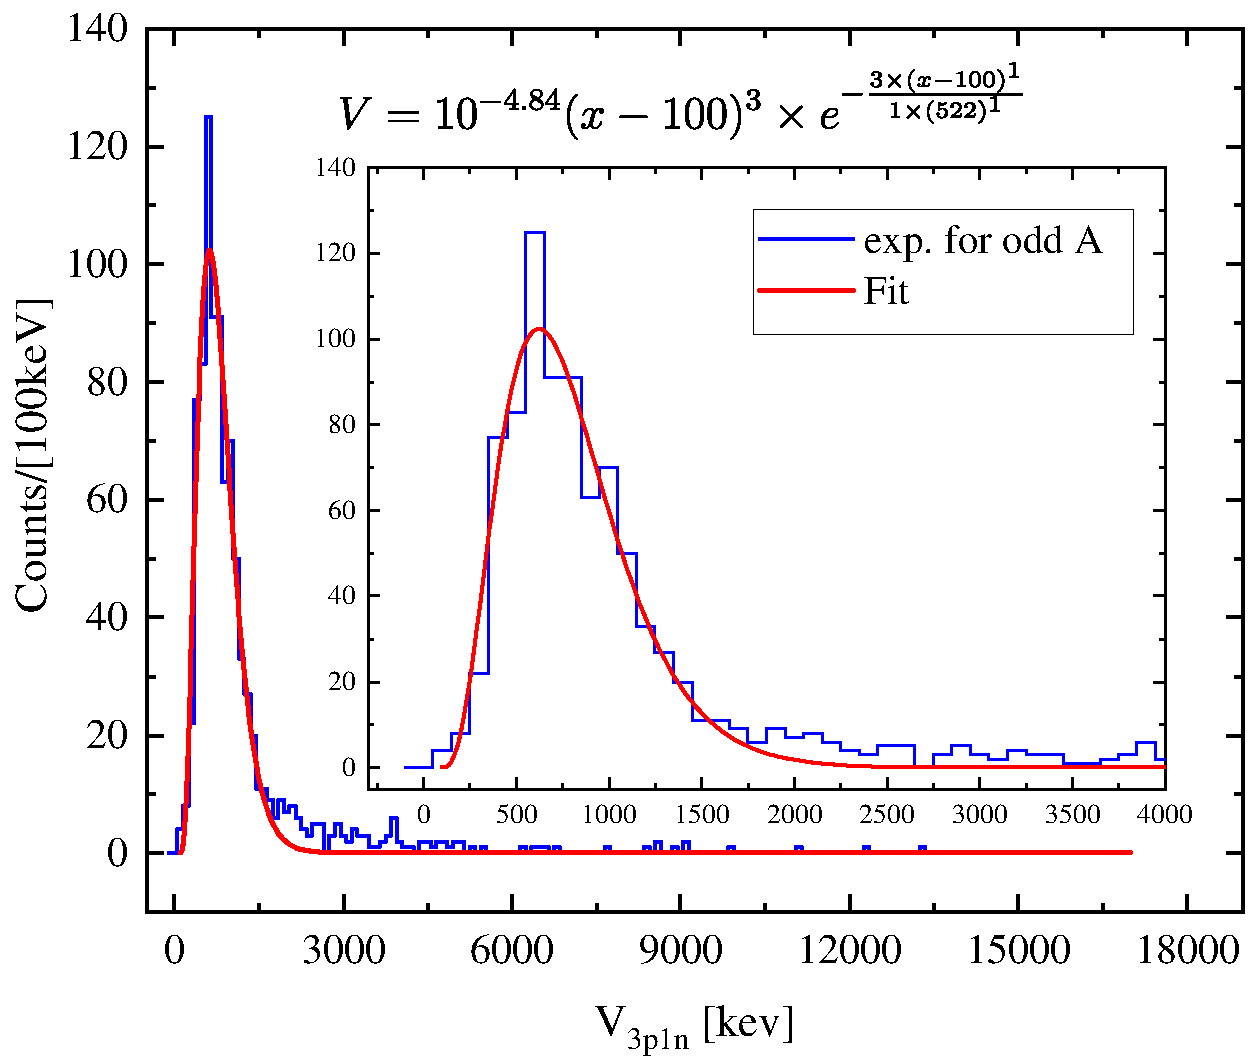
\includegraphics[width=0.4\textwidth]{figure/YE3fiteV3p1noA100.pdf}}
\caption{利用公式\ref{eq_fit}对AME2016的$V_{3p-1n}(Z,N)$相互作用的统计分布进行的拟合.\label{fig_YE3FitV3p1n_1}}
\end{figure}
\begin{figure}[H]
\centering
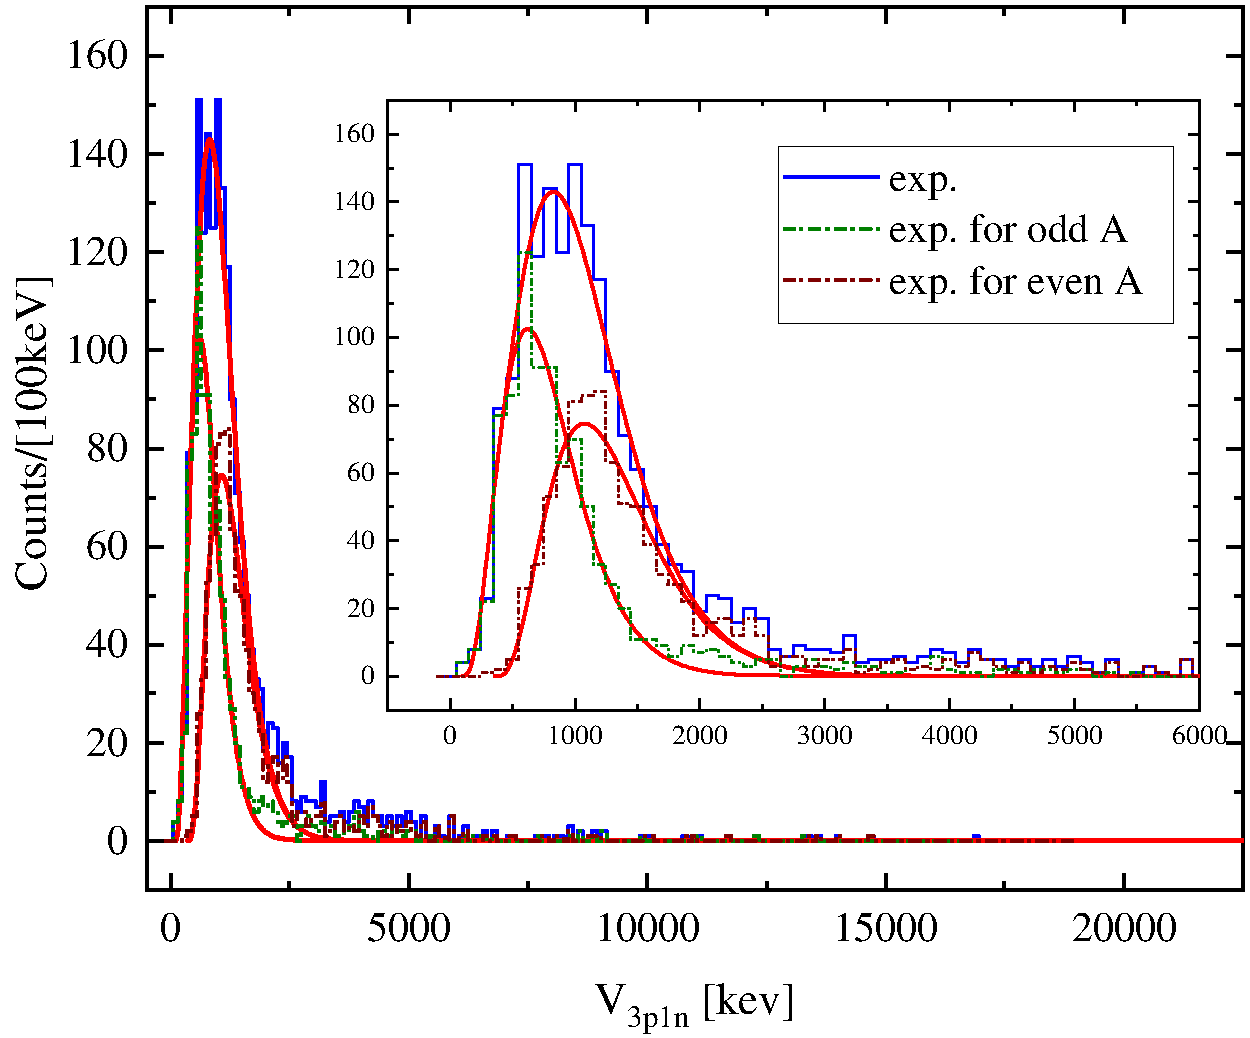
\includegraphics[width=0.6\textwidth]{figure/YE3fiteV3p1n100.pdf}
\caption{AME2016的奇A核的$V_{3p-1n}(Z,N)$相互作用的统计分布,以及拟合的结果.\label{fig_YE3fiteV3p1n100}}
\end{figure}

\begin{figure}[H]
\centering
\subfigure[利用公式\ref{eq_fit}对AME2016的偶A核的$V_{2p-2n}(Z,N)$相互作用进行的拟合.\label{fig_Y3FitV2p2neA100}]{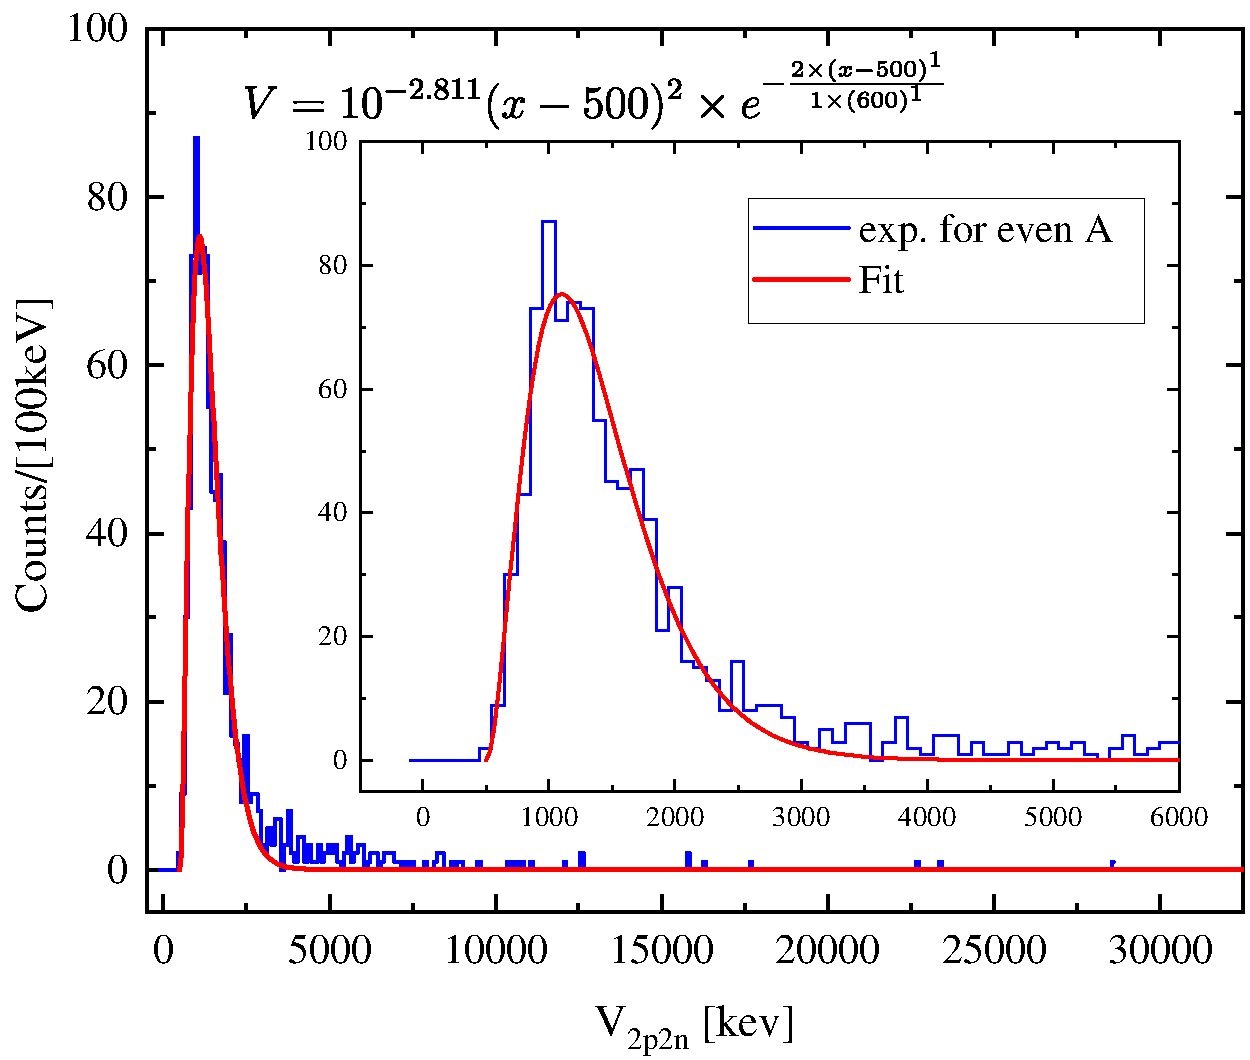
\includegraphics[width=0.4\textwidth]{figure/YE3fiteV2p2neA100.pdf}}
\qquad
\subfigure[利用公式\ref{eq_fit}对AME2016的奇A核的$V_{2p-2n}(Z,N)$相互作用进行的拟合.\label{fig_Y3FitV2p2noA100}]{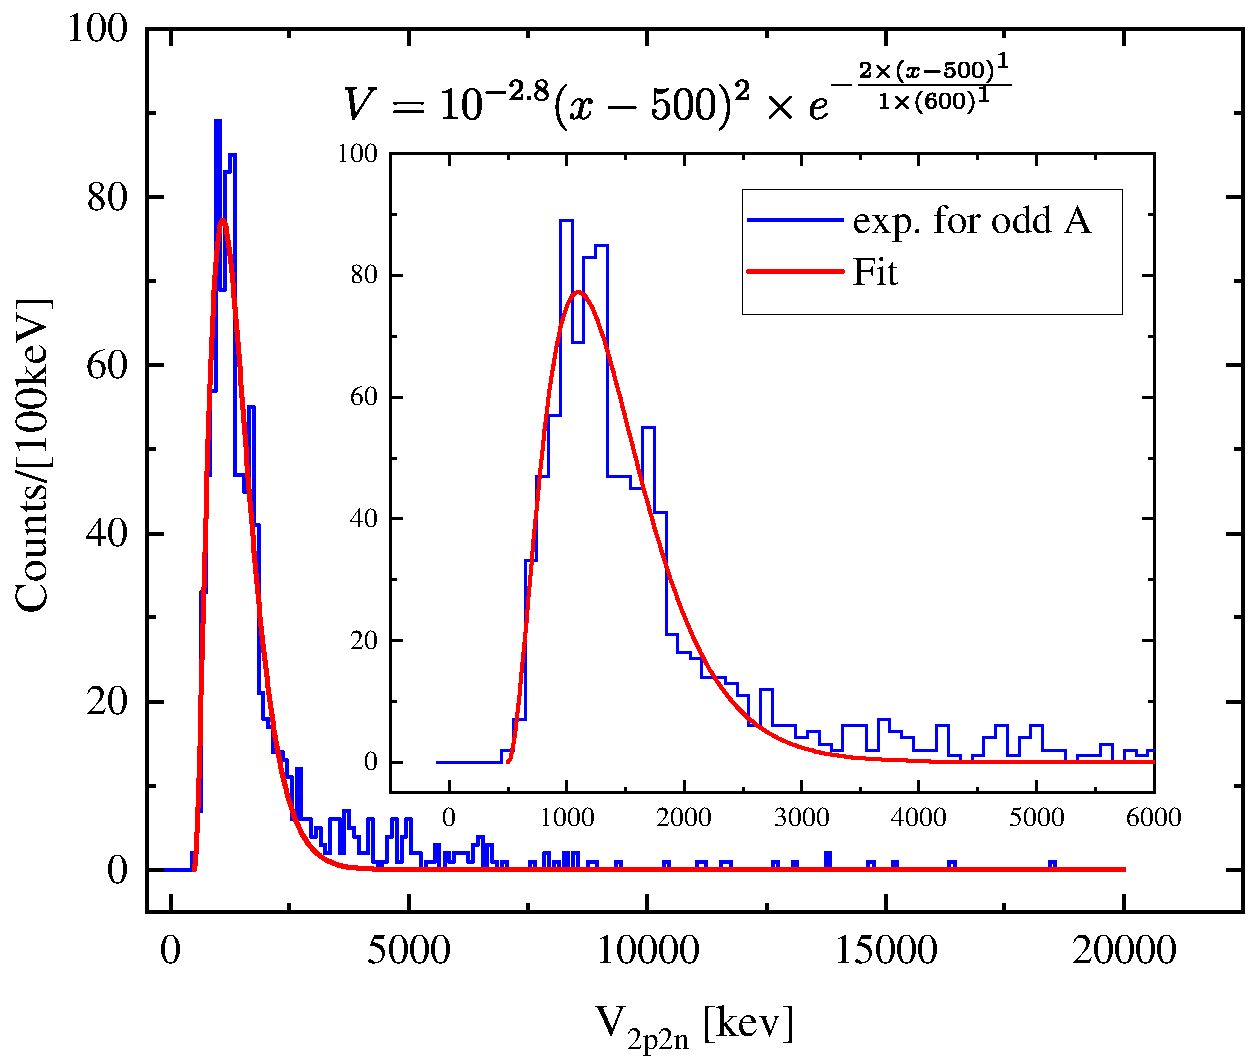
\includegraphics[width=0.4\textwidth]{figure/YE3fiteV2p2noA100.pdf}}
\caption{利用公式\ref{eq_fit}对AME2016的$V_{2p-2n}(Z,N)$相互作用的统计分布进行的拟合.\label{fig_YE3FitV2p2n_1}}
\end{figure}
\begin{figure}[H]
\centering
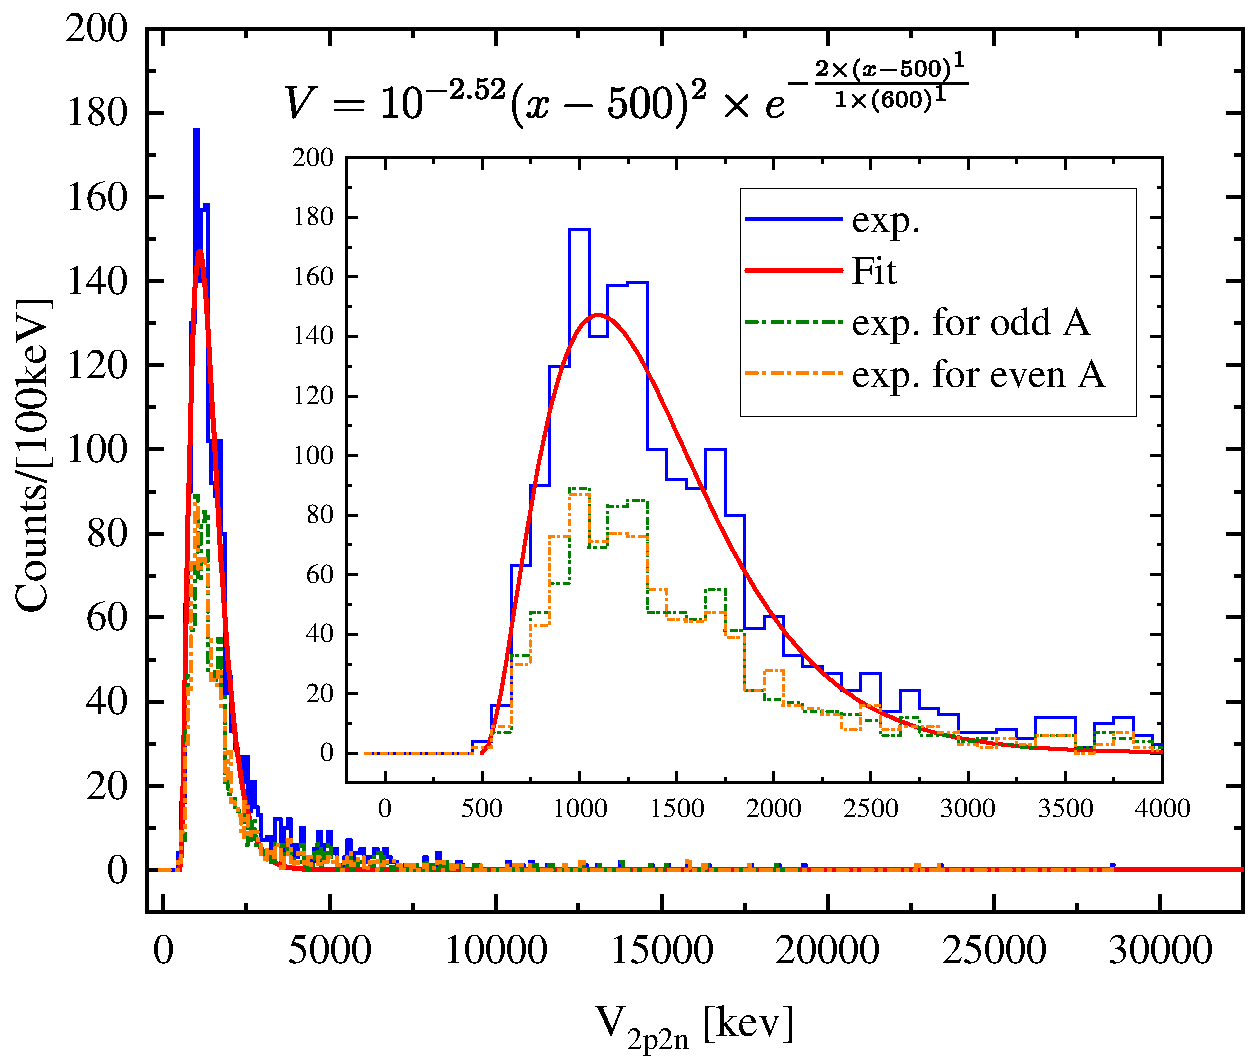
\includegraphics[width=0.6\textwidth]{figure/YE3fiteV2p2n100.pdf}
\caption{AME2016的奇A核的$V_{2p-2n}(Z,N)$相互作用的统计分布,以及拟合的结果.\label{fig_YE3fiteV2p2n100}}
\end{figure}
下面的表格给出了mass-date-based p-n相互作用的统计分布的所有拟合参数$a, b,c,d,f$:

% \begin{center}
% %
% \tablefirsthead{\hline\hline
% Interaction&Range&a&b&c&d&f\\\hline}
% \tablelasttail{\hline}
% %
% \tablehead{\hline\hline\multicolumn{7}{c}
% {\small\sl continued from previous page}\\\hline
% Interaction&Range&a&b&c&d&f\\\hline}
% \tabletail{\hline\hline}
 
% \begin{supertabular}{c|c|c c c c c}
% \multirow{3}*{$V_{1p-1n}(Z,N)$}&for even A& & & & &\\\cline{2-7}
% &for odd A& & & & &\\\cline{2-7}
% &for all nuclides& & & & &\\
% \hline
% \multirow{3}*{$V_{1p-2n}(Z,N)$}&for even A& & & & &\\\cline{2-7}
% &for odd A& & & & &\\\cline{2-7}
% &for all nuclides& & & & &\\
% \hline
% \multirow{3}*{$V_{2p-1n}(Z,N)$}&for even A& & & & &\\\cline{2-7}
% &for odd A& & & & &\\\cline{2-7}
% &for all nuclides& & & & &\\
% \hline
% \multirow{3}*{$V_{1p-3n}(Z,N)$}&for even A& & & & &\\\cline{2-7}
% &for odd A& & & & &\\\cline{2-7}
% &for all nuclides& & & & &\\
% \hline
% \multirow{3}*{$V_{3p-1n}(Z,N)$}&for even A& & & & &\\\cline{2-7}
% &for odd A& & & & &\\\cline{2-7}
% &for all nuclides& & & & &\\
% \hline
% \multirow{3}*{$V_{2p-2n}(Z,N)$}&for even A& & & & &\\\cline{2-7}
% &for odd A& & & & &\\\cline{2-7}
% &for all nuclides& & & & &\\
% \hline\hline
% \end{supertabular}
% \end{center}

\begin{table}[H]
\centering
\caption{mass-date-based p-n相互作用的统计分布的公式\ref{eq_fit}拟合参数}
\begin{tabular}{c|c|c c c c c}
\hline\hline
Interaction&Range&a&b&c&d&f\\
\hline\hline
\multirow{3}*{$V_{1p-1n}(Z,N)$}&for even A&4.64&490&80&3&1\\\cline{2-7}
&for odd A&10.56&90&-400&5&3\\\cline{2-7}
&for all nuclides&- -&- -&- -&- -&- -\\
\hline\hline
\multirow{3}*{$V_{1p-2n}(Z,N)$}&for even A&4.64&550&150&3&1\\\cline{2-7}
&for odd A&4.76&570&140&3&1\\\cline{2-7}
&for all nuclides&4.44&570&140&3&1\\
\hline\hline
\multirow{3}*{$V_{2p-1n}(Z,N)$}&for even A&4.76&560&130&3&1\\\cline{2-7}
&for odd A&2.35&530&200&2&1\\\cline{2-7}
&for all nuclides&2.05&530&200&2&1\\
\hline\hline
\multirow{3}*{$V_{1p-3n}(Z,N)$}&for even A&8.04&1080&250&4&1\\\cline{2-7}
&for odd A&7.36&655&45&4&1\\\cline{2-7}
&for all nuclides&- -&- -&- -&- -&- -\\
\hline\hline
\multirow{3}*{$V_{3p-1n}(Z,N)$}&for even A&5.36&1077&377&3&1\\\cline{2-7}
&for odd A&4.84&622&100&3&1\\\cline{2-7}
&for all nuclides&- -&- -&- -&- -&- -\\
\hline\hline
\multirow{3}*{$V_{2p-2n}(Z,N)$}&for even A&2.811&1100&500&2&1\\\cline{2-7}
&for odd A&2.8&1100&500&2&1\\\cline{2-7}
&for all nuclides&2.52&1100&500&2&1\\
\hline\hline
\end{tabular}
\end{table}
\noindent 从这个表格我们可以看出mass-date-based p-n相互作用的统计分布的一些特征:
\begin{enumerate}
  \item $V_{ip-jn}(Z,N)(i,j\ne0)$的统计分布与$V_{jp-in}(Z,N)$的统计分布非常相似;
  \item 对于$V_{ip-jn}(Z,N)(i,j\ne0)$,当${\rm mod}(i\times j,2)=0$时,偶A核与奇A核的统计分布基本相同;而当${\rm mod}(i\times j,2)\ne0$时,$i$偶A核与奇A核的统计分布存在奇偶差异,且偶A核的平均相互作用能更大,另外$i\times j$的值越小,奇偶差异越明显;
\end{enumerate}